\documentclass[a4paper,11pt]{book}
%\documentclass[a4paper,twoside,11pt,titlepage]{book}
\usepackage{listings}
\usepackage[utf8]{inputenc}
\usepackage[spanish,es-noshorthands]{babel}

% \usepackage[style=list, number=none]{glossary} %
%\usepackage{titlesec}
%\usepackage{pailatino}

\decimalpoint
\usepackage{dcolumn}
\newcolumntype{.}{D{.}{\esperiod}{-1}}
\makeatletter
\addto\shorthandsspanish{\let\esperiod\es@period@code}
\makeatother


%\usepackage[chapter]{algorithm}
\RequirePackage{verbatim}
%\RequirePackage[Glenn]{fncychap}
\usepackage{fancyhdr}
\usepackage{graphicx}
\usepackage{afterpage}

%%% PAQUETES AÑADIDOS POR MI
\usepackage{color}
\usepackage{xcolor}
\usepackage{caption}
\usepackage{subcaption}
\usepackage{float} % para dejar las imágenes fijas en un sitio
\usepackage{tikz}

\usepackage{longtable}

\usepackage[pdfborder={000}]{hyperref} %referencia

% ********************************************************************
% Re-usable information
% ********************************************************************
\newcommand{\myTitle}{Análisis de procesos\xspace}
\newcommand{\myDegree}{Grado en ...\xspace}
\newcommand{\myName}{María Isabel Ruiz Martínez (alumno)\xspace}
\newcommand{\myProf}{Luis Castillo Vidal (tutor1)\xspace}
\newcommand{\myOtherProf}{Nombre Apllido1 Apellido2 (tutor2)\xspace}
%\newcommand{\mySupervisor}{Put name here\xspace}
\newcommand{\myFaculty}{Escuela Técnica Superior de Ingenierías Informática y de
Telecomunicación\xspace}
\newcommand{\myFacultyShort}{E.T.S. de Ingenierías Informática y de
Telecomunicación\xspace}
\newcommand{\myDepartment}{Departamento de ...\xspace}
\newcommand{\myUni}{\protect{Universidad de Granada}\xspace}
\newcommand{\myLocation}{Granada\xspace}
\newcommand{\myTime}{\today\xspace}
\newcommand{\myVersion}{Version 0.1\xspace}


\hypersetup{
pdfauthor = {\myName (email (en) ugr (punto) es)},
pdftitle = {\myTitle},
pdfsubject = {},
pdfkeywords = {palabra_clave1, palabra_clave2, palabra_clave3, ...},
pdfcreator = {LaTeX con el paquete ....},
pdfproducer = {pdflatex}
}

%\hyphenation{}


%\usepackage{doxygen/doxygen}
%\usepackage{pdfpages}
\usepackage{url}
\usepackage{colortbl,longtable}
\usepackage[stable]{footmisc}
%\usepackage{index}

%\makeindex
%\usepackage[style=long, cols=2,border=plain,toc=true,number=none]{glossary}
% \makeglossary

% Definición de comandos que me son tiles:
%\renewcommand{\indexname}{Índice alfabético}
%\renewcommand{\glossaryname}{Glosario}

\pagestyle{fancy}
\fancyhf{}
\fancyhead[LO]{\leftmark}
\fancyhead[RE]{\rightmark}
\fancyhead[RO,LE]{\textbf{\thepage}}
\renewcommand{\chaptermark}[1]{\markboth{\textbf{#1}}{}}
\renewcommand{\sectionmark}[1]{\markright{\textbf{\thesection. #1}}}

\setlength{\headheight}{1.5\headheight}

\newcommand{\HRule}{\rule{\linewidth}{0.5mm}}
%Definimos los tipos teorema, ejemplo y definición podremos usar estos tipos
%simplemente poniendo \begin{teorema} \end{teorema} ...
\newtheorem{teorema}{Teorema}[chapter]
\newtheorem{ejemplo}{Ejemplo}[chapter]
\newtheorem{definicion}{Definición}[chapter]

\definecolor{gray97}{gray}{.97}
\definecolor{gray75}{gray}{.75}
\definecolor{gray45}{gray}{.45}
\definecolor{gray30}{gray}{.94}

\lstset{ frame=Ltb,
     framerule=0.5pt,
     aboveskip=0.5cm,
     framextopmargin=3pt,
     framexbottommargin=3pt,
     framexleftmargin=0.1cm,
     framesep=0pt,
     rulesep=.4pt,
     backgroundcolor=\color{gray97},
     rulesepcolor=\color{black},
     %
     stringstyle=\ttfamily,
     showstringspaces = false,
     basicstyle=\scriptsize\ttfamily,
     commentstyle=\color{gray45},
     keywordstyle=\bfseries,
     %
     numbers=left,
     numbersep=6pt,
     numberstyle=\tiny,
     numberfirstline = false,
     breaklines=true,
   }
 
% minimizar fragmentado de listados
\lstnewenvironment{listing}[1][]
   {\lstset{#1}\pagebreak[0]}{\pagebreak[0]}

\lstdefinestyle{CodigoC}
   {
	basicstyle=\scriptsize,
	frame=single,
	language=C,
	numbers=left
   }
\lstdefinestyle{CodigoC++}
   {
	basicstyle=\small,
	frame=single,
	backgroundcolor=\color{gray30},
	language=C++,
	numbers=left
   }

 
\lstdefinestyle{Consola}
   {basicstyle=\scriptsize\bf\ttfamily,
    backgroundcolor=\color{gray30},
    frame=single,
    numbers=none
   }


\newcommand{\bigrule}{\titlerule[0.5mm]}


%Para conseguir que en las páginas en blanco no ponga cabecerass
\makeatletter
\def\clearpage{%
  \ifvmode
    \ifnum \@dbltopnum =\m@ne
      \ifdim \pagetotal <\topskip
        \hbox{}
      \fi
    \fi
  \fi
  \newpage
  \thispagestyle{empty}
  \write\m@ne{}
  \vbox{}
  \penalty -\@Mi
}
\makeatother

\usepackage{pdfpages}
\begin{document}

\begin{titlepage}
 
 
\newlength{\centeroffset}
\setlength{\centeroffset}{-0.5\oddsidemargin}
\addtolength{\centeroffset}{0.5\evensidemargin}
\thispagestyle{empty}

\noindent\hspace*{\centeroffset}\begin{minipage}{\textwidth}

\centering

\includegraphics[width=0.9\textwidth]{imagenes/logos/logo_ugr.jpg}%\\[1.4cm]

\textsc{ \Large TRABAJO FIN DE GRADO\\[0.2cm]}
\textsc{ INGENIERÍA EN ...}\\[1cm]
% Upper part of the page
% 
% Title
{\Huge\bfseries Análisis de procesos\\
}
\noindent\rule[-1ex]{\textwidth}{3pt}\\[3.5ex]
{\large\bfseries Subtitulo del Proyecto}
\end{minipage}

\vspace{2.5cm}
\noindent\hspace*{\centeroffset}\begin{minipage}{\textwidth}
\centering

\textbf{Autor}\\ {María Isabel Ruiz Martínez (alumno)}\\[2.5ex]
\textbf{Directores}\\
{Luis Castillo Vidal (tutor1)\\
Nombre Apellido1 Apellido2 (tutor2)}\\[2cm]

\includegraphics[width=0.3\textwidth]{imagenes/logos/etsiit_logo.png}\\[0.1cm]
\textsc{Escuela Técnica Superior de Ingenierías Informática y de Telecomunicación}\\
\textsc{---}\\
Granada, mes de 201
\end{minipage}
%\addtolength{\textwidth}{\centeroffset}
%\vspace{\stretch{2}}
\end{titlepage}



\chapter*{}
%\thispagestyle{empty}
%\cleardoublepage

%\thispagestyle{empty}

%\begin{titlepage}
 
 
\setlength{\centeroffset}{-0.5\oddsidemargin}
\addtolength{\centeroffset}{0.5\evensidemargin}
\thispagestyle{empty}

\noindent\hspace*{\centeroffset}\begin{minipage}{\textwidth}

\centering
%
\includegraphics[width=0.9\textwidth]{imagenes/logo_ugr.jpg}\\[1.4cm]

%\textsc{ \Large PROYECTO FIN DE CARRERA\\[0.2cm]}
%\textsc{ INGENIERÍA EN INFORMÁTICA}\\[1cm]
% Upper part of the page
% 

 \vspace{3.3cm}

%si el proyecto tiene logo poner aquí

\includegraphics{imagenes/logo.png} 
 \vspace{0.5cm}

% Title

{\Huge\bfseries Análisis de procesos\\
}
\noindent\rule[-1ex]{\textwidth}{3pt}\\[3.5ex]
{\large\bfseries Subtítulo del proyecto.\\[4cm]}
\end{minipage}

\vspace{2.5cm}
\noindent\hspace*{\centeroffset}\begin{minipage}{\textwidth}
\centering

\textbf{Autor}\\ {María Isabel Ruiz Martínez (alumno)}\\[2.5ex]
\textbf{Directores}\\
{Luis Castillo Vidal (tutor1)\\
Nombre Apellido1 Apellido2 (tutor2)}\\[2cm]
%
\includegraphics[width=0.15\textwidth]{imagenes/tstc.png}\\[0.1cm]
%\textsc{Departamento de Teoría de la Señal, Telemática y Comunicaciones}\\
%\textsc{---}\\
%Granada, mes de 201
\end{minipage}
%\addtolength{\textwidth}{\centeroffset}
\vspace{\stretch{2}}

 
\end{titlepage}






\cleardoublepage
\thispagestyle{empty}

\begin{center}
{\large\bfseries Análisis de procesos: Subtítulo del proyecto}\\
\end{center}
\begin{center}
María Isabel Ruiz Martínez\\
\end{center}

%\vspace{0.7cm}
\noindent{\textbf{Palabras clave}: palabra\_clave1, palabra\_clave2, palabra\_clave3, ......}\\

\vspace{0.7cm}
\noindent{\textbf{Resumen}}\\

Poner aquí el resumen.
\cleardoublepage


\thispagestyle{empty}


\begin{center}
{\large\bfseries Project Title: Project Subtitle}\\
\end{center}
\begin{center}
First name, Family name (student)\\
\end{center}

%\vspace{0.7cm}
\noindent{\textbf{Keywords}: Keyword1, Keyword2, Keyword3, ....}\\

\vspace{0.7cm}
\noindent{\textbf{Abstract}}\\

Write here the abstract in English.

\chapter*{}
\thispagestyle{empty}

\noindent\rule[-1ex]{\textwidth}{2pt}\\[4.5ex]

Yo, \textbf{María Isabel Ruiz Martínez}, alumno de la titulación Doble Grado en Ingeniería Informática y Matemáticas de la \textbf{Escuela Técnica Superior
de Ingenierías Informática y de Telecomunicación de la Universidad de Granada}, con DNI 75576979Z, autorizo la
ubicación de la siguiente copia de mi Trabajo Fin de Grado en la biblioteca del centro para que pueda ser
consultada por las personas que lo deseen.

\vspace{6cm}

\noindent Fdo: María Isabel Ruiz Martínez

\vspace{2cm}

\begin{flushright}
Granada a X de junio de 2023.
\end{flushright}


\chapter*{}
\thispagestyle{empty}

\noindent\rule[-1ex]{\textwidth}{2pt}\\[4.5ex]

D. \textbf{Luis Castillo Vidal}, Catedrático de Universidad del Departamento de Ciencias de la Computación e Inteligencia Artificial de la Universidad de Granada.

%\vspace{0.5cm}

%D. \textbf{Nombre Apellido1 Apellido2 (tutor2)}, Profesor del Área de XXXX del Departamento YYYY de la Universidad de Granada.


\vspace{0.5cm}

\textbf{Informa:}

\vspace{0.5cm}

Que el presente trabajo, titulado \textit{\textbf{Análisis de procesos, Subtítulo del proyecto}},
ha sido realizado bajo su supervisión por \textbf{María Isabel Ruiz Martínez (alumno)}, y autorizamos la defensa de dicho trabajo ante el tribunal
que corresponda.

\vspace{0.5cm}

Y para que conste, expiden y firman el presente informe en Granada a X de mes de junio 2023.

\vspace{1cm}

\textbf{El director:}

\vspace{5cm}

\noindent \textbf{Luis Castillo Vidal}

\chapter*{Agradecimientos}
\thispagestyle{empty}

       \vspace{1cm}


Poner aquí agradecimientos...



\frontmatter
\tableofcontents
\listoffigures
\listoftables

\mainmatter
\setlength{\parskip}{5pt}

\chapter{Introducción, motivaciones, objetivos y estructura}
	\label{chap:one}
    
\section{Introducción}
\documentclass[10pt,a4paper]{article}
\usepackage[utf8]{inputenc}
\usepackage{amsmath}
\usepackage{amsfonts}
\usepackage{amssymb}
\usepackage{graphicx}
\usepackage[hidelinks]{hyperref} 
\usepackage{color}
\usepackage{xcolor}
\usepackage{caption}
\usepackage{subcaption}
\author{María Isabel Ruiz Martínez}
\title{Introducción}

%Ruta absoluta en formato tipo Unix (Linux, OsX)
\graphicspath{ {/home/maribel/Escritorio/5º DGIIM/TFG/Analysis-of-processes/documentation/images} }

\begin{document}

\maketitle

La necesidad de comprender el proceso de aprendizaje y de personalizar la enseñanza para realizar una mejor adaptación a las necesidades del individuo ha motivado la \emph{Analítica de Aprendizaje} o \emph{Learning Analytics}, disciplina que consiste en la recogida de datos de un entorno de aprendizaje y el análisis de los mismos cuyo objetivo es asistir en el proceso de aprendizaje del alumnado.

Además, el uso de laboratorios virtuales y remotos en la enseñanza está en auge. Entre muchas de sus ventajas tenemos una mayor privacidad para el alumnado, accesos planficados a los mismos o soporte para reportar la actividad de los alumnos y la calificación de los mismos.

En este trabajo fin de grado se usarán datos de cinco cursos académicos obtenidos en el labotorio virtual para sistemas multiagente de la asignatura del cuarto curso académico Desarrollo Basado en Agentes del grado de Ingeniería Informática de la Universidad de Granada (España).

El laboratorio virtual diseñado para la asignatura recoge el trabajo diario de los alumnos almacenando las interacción entre los diferentes agentes y obteniendo así un extenso dataset que nos proporciona una base sólida para el uso de diversas analíticas de aprendizaje.

Así pues, se empleará un enfoque \emph{``data-driven''} o \emph{impulsado por datos}, tomando decisiones estratégicas basándose en el análisis de los datos y en la interpretación de los mismos.

\end{document}

\section{Motivaciones}
\chapter*{Motivación}\label{sec:motivation}
\addcontentsline{toc}{chapter}{Motivación}

\section{Introducción}

La necesidad de comprender el proceso de aprendizaje y de personalizar la enseñanza para realizar una mejor adaptación a las necesidades del individuo ha motivado la \emph{Analítica de Aprendizaje} o \emph{Learning Analytics}, disciplina que consiste en la recogida de datos de un entorno de aprendizaje y el análisis de los mismos cuyo objetivo es asistir en el proceso de aprendizaje del alumnado.

Además, el uso de laboratorios virtuales y remotos en la enseñanza está en auge. Entre muchas de sus ventajas tenemos una mayor privacidad para el alumnado, accesos planificados a los mismos o soporte para reportar la actividad de los alumnos y la calificación de los mismos.

En este trabajo fin de grado se usarán datos de siete cursos académicos obtenidos en el laboratorio virtual para sistemas multiagente de la asignatura del cuarto curso académico Desarrollo Basado en Agentes del grado de Ingeniería Informática de la Universidad de Granada (España).

El laboratorio virtual diseñado para la asignatura recoge el trabajo diario de los alumnos almacenando las interacción entre los diferentes agentes y obteniendo así un extenso dataset que nos proporciona una base sólida para el uso de diversas analíticas de aprendizaje.

Así pues, se empleará un enfoque \emph{``data-driven''} o \emph{impulsado por datos}, tomando decisiones estratégicas basándose en el análisis de los datos y en la interpretación de los mismos.

\section{Motivación}

La principal motivación de este trabajo fin de grado es, precisamente, el análisis de los procesos de aprendizaje que siguen los alumnos para que el profesorado pueda asistirles mejor durante su proceso de aprendizaje y mejorar así su rendimiento académico.

Detectar grupos con dificultades para superar sus tareas de laboratorio es primordial para que el profesor pueda ayudarles y, cuanto antes, mejor. En este caso, el uso de técnicas de minería de procesos, comúnmente asociadas a indicadores de rendimiento de los alumnos, para extraer su comportamiento de un laboratorio virtual y la utilización de aprendizaje automático supervisado para identificar estos comportamientos han demostrado ser las herramientas fundamentales para identificar el comportamiento de los alumnos y prever grupos en riesgo. Así pues, en este estudio se demuestra que los indicadores de rendimiento de los alumnos pueden ser muy útiles, tanto como su comportamiento, estrictamente desde un punto de vista topológico.

\section{Objetivos}

Los objetivos principales del proyecto serán:
\begin{itemize}
\item Identificar patrones de comportamiento indicativos de la evolución de los alumnos y del progreso de su aprendizaje, detectando, en las fases más tempranas posibles, comportamientos que pudiesen ser anómalos o que pudiesen indicar problemas de aprendizaje. Es decir, se pretende relevar, mediante la utilización de técnicas de minería de procesos, las posibles estrategias de los alumnos para cumplir los distintos objetivos de la asignatura así como desvelar su forma de trabajo habitual.
\item Sugerir a estos alumnos las medidas necesarias para que recuperen un buen ritmo de aprendizaje y un progreso adecuado a lo que el profesorado de la asignatura espera.
\end{itemize}

\section{Estructura del Trabajo Fin de Grado}

Este trabajo fin de grado consta de seis partes, $16$ capítulos y otros elementos como la portada, la declaración de originalidad, la autorización para su ubicación en la biblioteca de la escuela, sendos resúmenes tanto en español como en inglés (con sus respectivas palabras clave), la sección de agradecimientos, el índice general así como de una bibliografía y un apéndice.

A continuación se expone un breve esquema general del contenido de las partes y capítulos de este trabajo fin de grado:

\begin{itemize}
\item \hyperref[sec:parteI]{Parte I}: Motivaciones.
\begin{itemize}
\item \hyperref[sec:motivation]{\emph{Motivación}}: Se trata de un capítulo inicial en el que se expone una introducción en el contexto del proyecto junto con las motivaciones existentes, los objetivos que se pretenden conseguir con la realización del mismo y la estructuración de la memoria.
\end{itemize}
\item \hyperref[sec:parteII]{Parte II}: Estado del arte.
\begin{itemize}
\item \hyperref[sec:chapterI]{Capítulo 1}: Planteamiento del problema. Describe el funcionamiento de la plataforma educativa que recoge los datos que se usarán en este trabajo fin de grado y la clase de tareas que se le platean al alumnado que hace uso de la misma. Igualmente, se presenta un ejemplo fictio que refleja el tipo de información recogida de la actividad de los alumnos.
\item \hyperref[sec:chapterII]{Capítulo 2}: Introducción a la Minería de Procesos y trabajos previos. Introducción al concepto clave de minería de procesos en relación a los objetivos que se plantean en este proyecto. Adicionalmente, se realiza una breve presentación de los estudios en este área previos a este trabajo y se realiza una clasificación de los trabajos realizados en el campo de la Minería de Procesos.
\item \hyperref[sec:chapterIII]{Capítulo 3}: Minería de Procesos. Breve descripción de la suite de minería de procesos Disco \cite{gunther2012disco} y de su algoritmo subyacente (\emph{Fuzzy Miner} \cite{gunther2007fuzzy}). Igualmente, se muestran algunos diagramas extraídos con dicha herramienta y se exponen sus principales limitaciones.
\item \hyperref[sec:chapterIV]{Capítulo 4}: Implementación de la herramienta de Minería de Procesos \emph{Graph Miner}. Breve introducción a la manera en la que se representarán los grupos de prácticas en la herramienta de minería de procesos de creación propia \emph{Graph Miner}: la matriz característica de un grupo. Finalmente, se muestran los distintos gráficos que pueden obtenerse a partir de esta nueva herramienta.
\item \hyperref[sec:chapterV]{Capítulo 5}: Teoría de grafos. Definiciones básicas relativas a la teoría de grafos entre las que se encuentra el concepto de \emph{Grafo Dirigido Acíclico}, concepto clave en el desarrollo de este trabajo. Además, se incluye la exposición y demostración del Teorema de Kirchhoff, generalización de la fórmula de Cayley que será de gran utilidad en el cálculo del número de árboles de expansión de grafos conexos. El capítulo finaliza con la presentación de algunas medidas de propósito general que se usarán para realizar una clasificación de los distintos grupos de prácticas.
\end{itemize}
\item \hyperref[sec:parteIII]{Parte III}: Análisis descriptivo.
\begin{itemize}
\item \hyperref[sec:chapterVI]{Capítulo 6}: Los registros existentes.  Incluye una descripción de los registros existentes en el servidor. Se muestra el número de grupos estudiados cada año, el periodo de tiempo analizado cada año y el conjunto de problemas analizados cada año, estudiando la dificultad de los mismos. Por último, se realiza un análisis de la actividad registrada en el servidor.
\item \hyperref[sec:chapterVII]{Capítulo 7}: Hipótesis de estudio. Exposición de las principales métricas de calidad definidas sobre los registros de actividad de los alumnos que podrían permitir discernir qué grupos presentan una mayor dificultad para resolver los problemas de prácticas propuestos. Se realiza una subdivisión de las mismas en continuas y a posteriori.
\item \hyperref[chapter:rendimiento]{Capítulo 8}: Rendimiento observado de los alumnos. Descripción detallada y estudio estadístico de las medidas de rendimiento de los alumnos clásicas. Se estudiarán las variaciones de las distintas variables a lo largo de los años y la normalidad de las mismas. El objetivo de este capítulo es la familiarización del lector con algunas de las métricas de calidad que serán determinantes en la predicción de grupos en riesgo.
\end{itemize}
\item \hyperref[sec:parteIV]{Parte IV}: Planificación del proyecto.
\begin{itemize}
\item \hyperref[chapter:objetivos]{Capítulo 9}: Etapas del proyecto: división en objetivos. Se describen las iteraciones en las que se divide el proyecto siguiendo la metodología \emph{Scrum}.
\item \hyperref[chapter:sprints]{Capítulo 10}: Etapas del proyecto: división en sprints y seguimiento de los mismos. Se muestra la organización temporal del proyecto y el seguimiento del mismo mediante \emph{burndown charts}.
\end{itemize}
\item \hyperref[sec:parteV]{Parte V}: Resultados obtenidos.
\begin{itemize}
\item \hyperref[chapter:correlations]{Capítulo 11}: Análisis de las correlaciones entre las distintas métricas. Análisis de la correlación existente entre las métricas clásicas para cuantificar el rendimiento de los alumnos y la nota obtenida por los mismos. Además, se estudiarán las correlaciones entre las medidas de complejidad (características topológicas de los grafos que representan el proceso de resolución de los problemas) y la nota alcanzada por los alumnos al final de la práctica.
\item \hyperref[sec:chapterXII]{Capítulo 12}: Perfiles de estudiantes según su rendimiento. Aplicación de técnicas de clustering para agrupar a los alumnos en diferentes intervalos de calificaciones empleando diferentes métricas (medidas clásicas de rendimiento y topológicas).
\item \hyperref[sec:chapterXIII]{Capítulo 13}: Clasificación de los grupos de alumnos según su rendimiento. Utilización del clasificador estadístico C5.0 para generar un conjunto de reglas que se emplearán para poder decidir si el rendimiento de una determinada agrupación de estudiantes es más bajo de lo que debería. Además, se utilizará otro clasificador del mismo tipo para predecir el intervalo de notas en el que se encontraría un determinado grupo de alumnos.
\end{itemize}
\item \hyperref[sec:parteVI]{Parte VI}: Conclusiones y vías futuras.
\begin{itemize}
\item \hyperref[sec:chapterXIV]{Capítulo 14}: Conclusiones. Repaso de los logros alcanzados a lo largo del proyecto y recapitulación de la principal motivación del desarrollo de este trabajo.
\item \hyperref[sec:chapterXV]{Capítulo 15}: Vías futuras. Exposición de un conjunto de propuestas para ampliar el trabajo aquí realizado.
\end{itemize}
\end{itemize}

\section{Objetivos}
\chapter{Etapas del proyecto: división en objetivos}\label{chapter:objetivos}
\addcontentsline{toc}{chapter}{Etapas del proyecto: división en objetivos}

El proyecto se ha realizado siguiendo la metodología \emph{Scrum}
Durante la fase inicial de planificación del proyecto se realizó una subdivisión del mismo en iteraciones:
\begin{itemize}
\item Realización de un estudio multianual y segmentado por calificaciones y primeros resultados de homogeneidad de las muestras transversal por años mediante la realición de análisis ANOVA.
\item Extracción de procesos ocultos en los datasets utilizando el programa DISCO y programación y mejora del proceso de extracción. El resultado de esta fase serán una serie de grafos representando a cada uno de los grupos de prácticas considerados donde los arcos implican una relación de dependencia temporal. Estos grafos se representarán a partir de matrices de adyacencia cuyos vértices podrán representar problemas de prácticas, pares problema de prácticas y milestone alcanzado o pares problema de prácticas y estado (\texttt{FAIL} si no se ha resuelto el problema y \texttt{OK} en caso contrario).
\item Análisis de los procesos por distintas categorías: por años (resultando ser estadísticamente iguales) y por calificación final del grupo (resultando en la existencia de diferencias). Así pues, se pretenderá caracterizar el comportamiento de los grupos.
\item Análisis del comportamiento de un mismo grupo a lo largo del tiempo. Se realizará un estudio con el fin de determinar si el comportamiento de un grupo varía durante el desarrollo de las prácticas.
\end{itemize}

\section{Organización de este Trabajo Fin de Grado}
Este trabajo fin de grado consta de cuatro partes, siete capítulos y otros elementos como la portada, la autorización para su ubicación en la biblioteca de la escuela, sendos resúmenes tanto en español como en inglés (con sus respectivas palabras clave), la sección de agradecimientos, los índices general, de figuras y de cuadros así como una bibliografía, un glosario de términos y un glosario de acrónimos.

A continuación se expone un breve esquema general del contenido de las partes y capítulos de este trabajo fin de grado:

\begin{itemize}
\item Parte I:
\item Parte II:
\item Parte III:
\item Parte IV:
\end{itemize}

%
%\input{capitulos/02_EspecificacionRequisitos}
%
\chapter{Planificación}
    \label{chap:three}
   
\section{Herramientas}
\documentclass[10pt,a4paper]{article}
\usepackage[utf8]{inputenc}
\usepackage{amsmath}
\usepackage{amsfonts}
\usepackage{amssymb}
\usepackage{graphicx}
\usepackage[hidelinks]{hyperref} 
\usepackage{color}
\usepackage{xcolor}
\usepackage{caption}
\usepackage{subcaption}
\author{María Isabel Ruiz Martínez}
\title{Herramientas}

%Ruta absoluta en formato tipo Unix (Linux, OsX)
\graphicspath{ {/home/maribel/Escritorio/5º DGIIM/TFG/Analysis-of-processes/documentation/images} }

\begin{document}

\maketitle

En la realización de un proyecto investigación, la elección de las herramientas para su desarrollo es clave. A continuación se expone una lista con las que se han utilizado este trabajo fin de grado:

\begin{itemize}
	\item En el desarrollo del software se han empleado los lenguajes de
programación \texttt{R} y \texttt{C++}.
	\item Se ha empleado la herramienta de míneria de procesos \texttt{DISCO}.
	\item Se ha utilizado \texttt{GitHub} para alojar todo el 			contenido del proyecto y gestionar las distintas versiones del mismo.
	\item Para la redacción de la memoria se ha empleado el editor gratuito \texttt{Texmaker} utilizando el sistema de composición de textos \LaTeX.
	\item Para el seguimiento del proyecto se han utilizado las \texttt{Hojas de cálculo de Google}.
\end{itemize}

\end{document}


\chapter{Análisis}
	\label{chap:four}
	
\section{Planteamiento del problema}
El servidor contiene varios mundos virtuales. Cada mundo virtual es una matriz cuadrada que representa espacios abiertos (en color blanco), obstáculos (en negro) y objetivos (en rojo) tal y como se muestra en la Figura \ref{fig:1}. Los agentes de los alumnos deben entrar en uno de esos mundos virtuales, percibir su vecindario, navegar a través de los espacios abiertos (empleando alguna clase de heurística exploratoria), evitar obstáculos y tratar de llegar al objetivo.

La percepción del agente de su entorno es crítica para resolver estos mundos. En este laboratorio virtual los alumnos pueden configurar cuál de los siguientes sensores estarán enchufados en sus agentes (cualquier combinación de ellos):

\begin{itemize}
	\item Un \textbf{GPS} que indica al agente sus coordenadas $(x,y)$ en el mundo virtual.
	\item Un \textbf{sensor de batería}. Cada agente está alimentado con una batería cuya capacidad es limitada y cuya carga decrece conforme el agente realiza algún movimiento. La batería nunca debe ser vaciada por completo.
	\item Un \textbf{sensor radar} que informa al agente acerca de los tipos de celdas que lo rodean con una percepción local de 5x5 (observar Figura \ref{fig:2}).
	\item Un \textbf{sensor escáner} que actúa como \emph{detector del objetivo} e indica al agente la distancia al objetivo medida desde cada una las celdas de su entorno 5x5 (observar Figura \ref{fig:3}).
\end{itemize}

Basados en su percepción del mundo virtual, cada agente decidirá ejecutar alguna de las siguientes acciones en su entorno implementando cualquier heurística o proceso de búsqueda.

\begin{itemize}
	\item LOGIN. Entrar en cualquiera de los mundos virtuales.
	\item MOVE. Mover al agente a una de las $8$ celdas adyacentes y gastar una cierta cantidad de batería. Si la celda destino es un obstáculo o el agente se queda sin batería, el agente se rompe y se sale del mundo  virtual.
	\item REFUEL. El agente recarga completamente su batería. A los agentes se les permite recargar su batería tantas veces como deseen.
\end{itemize}
\section{Algunos conceptos relevantes}
En el ámbito de las matemáticas y las ciencias de la computación, se emplea el término \emph{``grafo''} (del griego \emph{``grafos''} que significa \emph{``dibujo''} o \emph{``imagen''}) para referirse a un conjunto de objetos llamados \emph{``vértices''} o \emph{``nodos''}, los cuales están unidos por enlaces conocidos como \emph{``aristas''} o \emph{``arcos''}. Estas conexiones representan las relaciones binarias que existen entre los elementos de un conjunto, y son objeto de estudio de la teoría de grafos.

En la Figura \ref{fig:grafo1} se muestra un ejemplo de grafo.

\begin{figure}[H]
\centering
\begin{tikzpicture}

% Posiciones fijas de los nodos
\node[circle, draw=black, fill=white] (A) at (0,0) {A};
\node[circle, draw=black, fill=white] (B) at (2,2) {B};
\node[circle, draw=black, fill=white] (C) at (2,-2) {C};
\node[circle, draw=black, fill=white] (D) at (-2,-2) {D};
\node[circle, draw=black, fill=white] (E) at (-2,2) {E};

% Arcos aleatorios
\draw[-, blue, line width=1pt] (A) to[bend left=20] (B);
\draw[-, green, line width=1pt] (B) to[bend left=20] (C);
\draw[-, red, line width=1pt] (C) to[bend left=20] (D);
\draw[-, orange, line width=1pt] (D) to[bend left=20] (E);
\draw[-, purple, line width=1pt] (E) to[bend left=20] (A);
\draw[-, violet, line width=1pt] (A) to[bend left=20] (C);

\end{tikzpicture}
\caption{Ejemplo de grafo con $5$ nodos.}
\label{fig:grafo1}
\end{figure}

Asimismo, se denomina \emph{grafo dirigido} o \emph{digrafo} a aquellos grafos cuyas aristas tengan un sentido definido. Por el contrario, las aristas de los grafos no dirigidos representan relaciones simétricas.

En la Figura \ref{fig:grafo2} se muestra un ejemplo de grafo dirigido.

\begin{figure}[H]
\centering
\begin{tikzpicture}

% Posiciones fijas de los nodos
\node[circle, draw=black, fill=white] (A) at (0,0) {A};
\node[circle, draw=black, fill=white] (B) at (2,2) {B};
\node[circle, draw=black, fill=white] (C) at (2,-2) {C};
\node[circle, draw=black, fill=white] (D) at (-2,-2) {D};
\node[circle, draw=black, fill=white] (E) at (-2,2) {E};

% Arcos aleatorios
\draw[->, blue, line width=1pt] (A) to[bend left=20] (B);
\draw[->, green, line width=1pt] (B) to[bend left=20] (C);
\draw[->, red, line width=1pt] (C) to[bend left=20] (D);
\draw[->, orange, line width=1pt] (D) to[bend left=20] (E);
\draw[->, purple, line width=1pt] (E) to[bend left=20] (A);
\draw[->, violet, line width=1pt] (A) to[bend left=20] (C);

\end{tikzpicture}
\caption{Ejemplo de grafo dirigido con $5$ nodos.}
\label{fig:grafo2}
\end{figure}

No obstante, en este trabajo fin de grado nos serán de gran utilidad los llamados \emph{grafos dirigidos acíclicos} o \emph{DAG} (\emph{Directed Acyclic Graphs}, en inglés) que no son más que grafos dirigidos desprovistos de ciclos.

En la Figura \ref{fig:grafo3} se muestra un ejemplo de grafo acíclico dirigido. Por el contrario, el grafo que se muestra en la figura \ref{fig:grafo2} no es acíclico (tiene ciclos, por ejemplo, el $A$-$C$-$D$-$E$).

\begin{figure}[H]
\centering
\begin{tikzpicture}

% Posiciones fijas de los nodos
\node[circle, draw=black, fill=white] (A) at (0,0) {A};
\node[circle, draw=black, fill=white] (B) at (2,2) {B};
\node[circle, draw=black, fill=white] (C) at (2,-2) {C};
\node[circle, draw=black, fill=white] (D) at (-2,-2) {D};
\node[circle, draw=black, fill=white] (E) at (-2,2) {E};

% Arcos aleatorios
\draw[->, blue, line width=1pt] (A) to[bend left=20] (B);
\draw[->, green, line width=1pt] (B) to[bend left=20] (C);
\draw[->, red, line width=1pt] (C) to[bend left=20] (D);
\draw[->, orange, line width=1pt] (D) to[bend left=20] (E);
\draw[->, violet, line width=1pt] (A) to[bend left=20] (C);

\end{tikzpicture}
\caption{Ejemplo de grafo acíclico dirigido con $5$ nodos.}
\label{fig:grafo3}
\end{figure}


\chapter{Diseño}
	\label{chap:five}
%
\chapter{Implementación}
	\label{chap:six}
	
\section{Análisis ANOVA y primeras conclusiones}
\subsection{Descripción del dataset}

Los datasets que se van a usar han sido recopilados por Luis Castillo Vidal y corresponden a la actividad de sus alumnos en la asignatura \href{https://www.ugr.es/estudiantes/grados/grado-ingenieria-informatica/desarrollo-basado-agentes-ing-software}{\color{blue}{Desarrollo Basado en Agentes}}.

El primer dataset, tras haber sido filtrados los registros erróneos, consta de 47828 filas correspondientes a los diferentes acciones de unos drones en una serie de mundos virtuales. En cada registro se detallan los siguientes atributos:
\begin{itemize}
\item \emph{year}: identifica el curso académico en el que se realizó dicha acción.
\item \emph{group}: grupo de prácticas que ha prograda al dron que acomete la acción.
\item \emph{date}: fecha en la que se lleva a cabo la acción.
\item \emph{map}: mundo virtual en el que se ha realizado la acción.
\item \emph{action}: indica el tipo de acción realizada.
\end{itemize}
% Dimesiones: 47828 registros, 5 columnas por registro.

En la Tabla \ref{table:1} se presentan los primeros seis registros del dataset. Además, en la Tabla \ref{table:2} puede apreciarse un resumen de los datos que tenemos.

% Muestra del dataset 1
% latex table generated in R 4.2.2 by xtable 1.8-4 package
% Wed Feb  1 15:07:17 2023
\begin{table}[ht]
\centering
\begin{tabular}{rlllll}
  \hline
 & year & group & date & map & action \\ 
  \hline
1 & 1516 & Achernar & 17/10/2015 19:41:45 & 0 & 0 \\ 
  2 & 1516 & Bellatrix & 17/10/2015 19:41:45 & 0 & 0 \\ 
  3 & 1516 & Cerastes & 17/10/2015 19:41:45 & 0 & 0 \\ 
  4 & 1516 & Denebola & 17/10/2015 19:41:45 & 0 & 0 \\ 
  5 & 1516 & Elnath & 17/10/2015 19:41:45 & 0 & 0 \\ 
  6 & 1516 & Furud & 17/10/2015 19:41:45 & 0 & 0 \\ 
   \hline
\end{tabular}
\caption{Muestra del primer dataset}
\label{table:1}
\end{table}

% Resumen del dataset que tenemos:
% latex table generated in R 4.2.2 by xtable 1.8-4 package
% Wed Feb  1 15:08:53 2023
\begin{table}[ht]
\centering
\begin{tabular}{lllll}
  \hline
     year &    group &     date &      map &     action \\ 
  \hline
Min.   :1516   & Length:47828       & Length:47828       & Min.   :0.000   & Min.   :0.000   \\ 
  1st Qu.:1516   & Class :character   & Class :character   & 1st Qu.:1.000   & 1st Qu.:1.000   \\ 
  Median :1617   & Mode  :character   & Mode  :character   & Median :3.000   & Median :2.000   \\ 
  Mean   :1700   &  &  & Mean   :3.834   & Mean   :2.325   \\ 
  3rd Qu.:1920   &  &  & 3rd Qu.:6.000   & 3rd Qu.:3.000   \\ 
  Max.   :1920   &  &  & Max.   :9.000   & Max.   :5.000   \\ 
   \hline
\end{tabular}
\caption{Resumen del primer dataset que tenemos}
\label{table:2}
\end{table}

La Figuras \ref{fig:boxplotmap} y \ref{fig:boxplotaction} muestran, respectivamente, los gráficos de caja y bigotes de las variables \emph{map} y \emph{action}.

\begin{figure}[!tbp]
  \begin{subfigure}[b]{0.49\textwidth}
    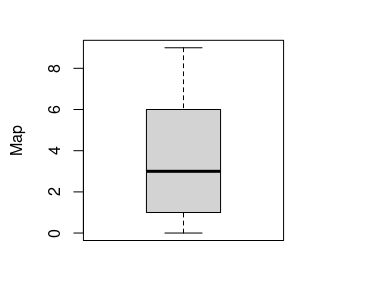
\includegraphics[width=\textwidth, height=\textwidth]{imagenes/Rplot02.png}
    \caption{Gráfico de caja y bigotes de la variable \emph{map}}
    \label{fig:boxplotmap}
  \end{subfigure}
  \hfill
  \begin{subfigure}[b]{0.49\textwidth}
    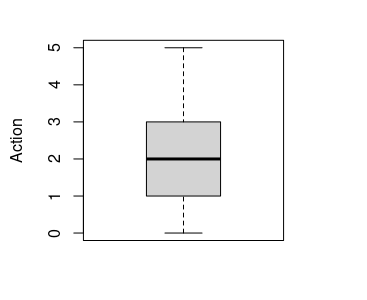
\includegraphics[width=\textwidth, height=\textwidth]{imagenes/Rplot04.png}
    \caption{Gráfico de caja y bigotes de la variable \emph{action}}
    \label{fig:boxplotaction}
  \end{subfigure}
  \caption{Diagramas de caja y bigotes de las variables \emph{map} y \emph{action}}
\end{figure}

Además, podemos ver la distribución de los diferentes niveles del factor \emph{map} y de los diferentes niveles del factor \emph{action} en las Figuras \ref{fig:yearmap} y \ref{fig:yearaction}.

\begin{figure}[!tbp]
  \begin{subfigure}[b]{0.49\textwidth}
    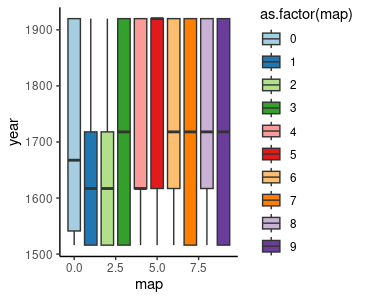
\includegraphics[width=\textwidth, height=\textwidth]{imagenes/Rplot.png}
    \caption{Distribución de los diferentes niveles del factor \emph{map}}
    \label{fig:yearmap}
  \end{subfigure}
  \hfill
  \begin{subfigure}[b]{0.49\textwidth}
    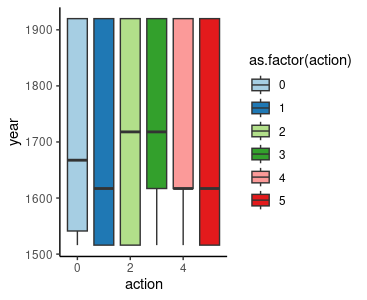
\includegraphics[width=\textwidth, height=\textwidth]{imagenes/Rplot01.png}
    \caption{Distribución de los diferentes niveles del factor \emph{action}}
    \label{fig:yearaction}
  \end{subfigure}
  \caption{Distribuciones para diferentes niveles de los factores}
\end{figure}

Por último, también podemos ver la distribución de las variables \emph{map} y \emph{action} en función del año (variable \emph{year}) en las Figuras \ref{fig:mapyear} y \ref{fig:actionyear}.

\begin{figure}[!tbp]
  \begin{subfigure}[b]{0.49\textwidth}
    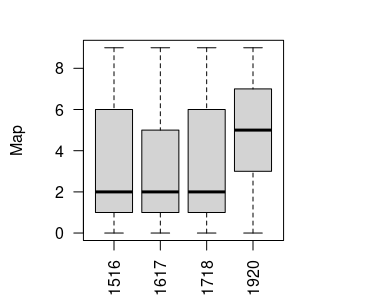
\includegraphics[width=\textwidth, height=\textwidth]{imagenes/Rplot03.png}
    \caption{Distribución de la variable \emph{map} en función de \emph{year}}
    \label{fig:mapyear}
  \end{subfigure}
  \hfill
  \begin{subfigure}[b]{0.49\textwidth}
    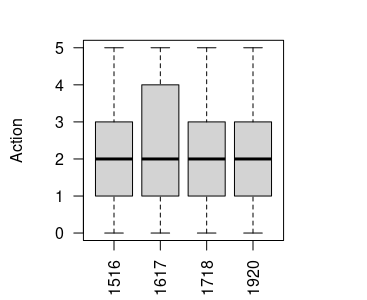
\includegraphics[width=\textwidth, height=\textwidth]{imagenes/Rplot05.png}
    \caption{Distribución de la variable \emph{action} en función de \emph{year}}
    \label{fig:actionyear}
  \end{subfigure}
  \caption{Distribuciones de las variables \emph{map} y \emph{action} dependiendo del valor de \emph{year}}
\end{figure}

El segundo dataset, tras haber sido eliminados algunas columnas que no eran interesantes para nuestro estudio, consta de 118 filas correspondientes a las diferentes calificaciones de los equipos en las dos prácticas realizadas en la asignatura \href{https://www.ugr.es/estudiantes/grados/grado-ingenieria-informatica/desarrollo-basado-agentes-ing-software}{\color{blue}{Desarrollo Basado en Agentes}}. En cada registro se detallan los siguientes atributos:
\begin{itemize}
\item \emph{Group}: grupo de prácticas que ha prograda al dron.
\item \emph{Team}: cadena de texto que identifica el curso académico en el que se realizó dicha acción, la práctica realizada y el grupo de prácticas conjuntamente.
\item \emph{Size}: tamaño del grupo de práctcas.
\item \emph{Year}: identifica el curso académico en el que se realizó dicha acción.
\item \emph{Grade}: calificación obtenida por el grupo de prácticas.
\end{itemize}
% Dimesiones: 118 registros, 5 columnas por registro.

En la Tabla \ref{table:6} se presentan los primeros seis registros del dataset. Además, en la Tabla \ref{table:7} puede apreciarse un resumen de los datos que tenemos.

% Muestra del dataset 2
% latex table generated in R 4.2.2 by xtable 1.8-4 package
% Sun Feb  5 13:27:02 2023
\begin{table}[ht]
\centering
\begin{tabular}{rlllll}
  \hline
 & Group & Team & Size & Year & Grade \\ 
  \hline
1 & G1 & DBA 1819 P3 GL & 4 & 1819 & 10,00 \\ 
  2 & G2 & DBA 1920 P3 GJ & 4 & 1920 & 4,01 \\ 
  3 & G3 & DBA 1819 P2 GH & 4 & 1819 & 7,96 \\ 
  4 & G4 & DBA 1920 P2 GE & 4 & 1920 & 8,95 \\ 
  5 & G5 & DBA 1920 P3 GK & 4 & 1920 & 4,51 \\ 
  6 & G6 & DBA 1415 P3 G6 & 6 & 1415 & 7,20 \\ 
   \hline
\end{tabular}
\caption{Muestra del segundo dataset}
\label{table:6}
\end{table}

% latex table generated in R 4.2.2 by xtable 1.8-4 package
% Sun Feb  5 13:31:46 2023
\begin{table}[ht]
\centering
\begin{tabular}{lllll}
  \hline
   Group &     Team &      Size &      Year &    Grade \\ 
  \hline
Length:118         & Length:118         & Min.   :3.000   & Min.   :1314   & Length:118         \\ 
  Class :character   & Class :character   & 1st Qu.:4.000   & 1st Qu.:1516   & Class :character   \\ 
  Mode  :character   & Mode  :character   & Median :5.000   & Median :1718   & Mode  :character   \\ 
   &  & Mean   :4.831   & Mean   :1662   &  \\ 
   &  & 3rd Qu.:6.000   & 3rd Qu.:1819   &  \\ 
   &  & Max.   :6.000   & Max.   :1920   &  \\ 
   \hline
\end{tabular}
\caption{Resumen del segundo dataset que tenemos}
\label{table:7}
\end{table}

\subsection{Introducción}

En este estudio inicial se desarrollará un modelo estadístico para determinar el efecto de los parámetros \emph{map} y \emph{action} (dos varibles explicativas) en la variable respuesta \emph{year}.

La relevancia de cada una de las variables en el modelo se determinará por el test \emph{two way ANOVA} con un $5\%$ de nivel de significancia y se empleará la técnica de los \emph{mínimos cuadrados} para estimar los coeficientes del modelo considerado.

\subsection{Two way ANOVA}

Un resumen de los resultados obtenidos al realizar el test two way ANOVA se muestra en la Tabla \ref{table:3}. Puede observarse que la variable \emph{map} es significante al nivel $0$, que la variable \emph{action} es significante al nivel $0.01$ y que la variable \emph{map:action} (el término de interacción) no es significante. Así pues, puede concluirse que el dataset es homógeneo, es decir, las combinaciones \emph{map:action} son estadísticamente iguales en todos los años considerados.

%Resumen two way ANOVA test:
% latex table generated in R 4.2.2 by xtable 1.8-4 package
% Wed Feb  1 15:19:36 2023
\begin{table}[ht]
\centering
\begin{tabular}{lrrrrr}
  \hline
 & Df & Sum Sq & Mean Sq & F value & Pr($>$F) \\ 
  \hline
map         & 1 & 62918413.58 & 62918413.58 & 2689.15 & 0.0000 \\ 
  action      & 1 & 101244.69 & 101244.69 & 4.33 & 0.0375 \\ 
  map:action  & 1 & 8797.03 & 8797.03 & 0.38 & 0.5398 \\ 
  Residuals   & 47824 & 1118946173.13 & 23397.17 &  &  \\ 
   \hline
\end{tabular}
\caption{Resultados del test two way ANOVA}
\label{table:3}
\end{table}

La notación escalar del modelo ajustado al aplicar el test tiene la siguiente estructura:

\begin{equation}
    y = \beta_0 + \beta_1 \cdot x_1 + \beta_2 \cdot x_2 + \beta_3 \cdot x_1 \cdot x_2 + \epsilon
\label{eq1}
\end{equation}

donde $\beta_0$ es el intercepto, $\beta_1$ y $\beta_2$ son los coeficientes de los efectos principales, $\beta_3$ es el coeficiente del término de interacción, $x_1$ y $x_2$ son los parámetros sometidos a investigación (en este caso, $x_1$ representa el parámetro mapa y $x_2$ representa la acción), $y$ representa el año y $\epsilon$ es el \emph{término error}.

La Tabla \ref{table:4} muestra los valores de los coeficientes de la fórmula que se han obtenido tras ajustar el modelo de regresión a los datos.

%Coeficientes del modelo:
% latex table generated in R 4.2.2 by xtable 1.8-4 package
% Wed Feb  1 15:20:53 2023
\begin{table}[ht]
\centering
\begin{tabular}{rr}
  \hline
 & x \\ 
  \hline
(Intercept) & 1655.03 \\ 
  map & 12.31 \\ 
  action & -1.51 \\ 
  map:action & 0.12 \\ 
   \hline
\end{tabular}
\caption{Coeficientes del modelo}
\label{table:4}
\end{table}

La Figura \ref{fig:interaccion} muestra la interacción entre los parámetros mapa y acción. Así pues, puede observarse que todas las líneras de la gráfica siguen más o menos el mismo patrón, lo que evidencia que no hay una gran interacción entre ambos.

\begin{figure}[h]
    \centering
    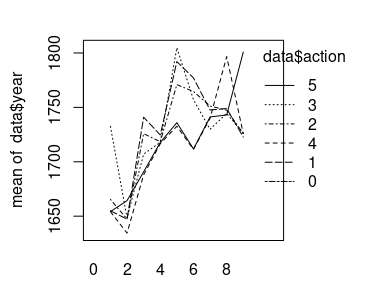
\includegraphics[width=0.60\textwidth]{imagenes/Rplot06.png}
    \caption{Interacción entre las variables \emph{map} y \emph{action}}
    \label{fig:interaccion}
\end{figure}

% Tukey multiple comparisons of means
% 95% family-wise confidence level
% Fit: aov(formula = year ~ map * action, data = data)
% $map

La Figura \ref{fig:suposiciones} muestra que no se violan las suposiciones que hemos realizado sobre el modelo. La media y la varianza de los residuos no parece que varíe respecto de los valores ajustados. Como consecuencia, conluiré que podemos suponer la homocedasticidad. Además, si nos fijamos en el \emph{Normal Q-Q plot}, puede observarse que los residuos son gaussianos.

\begin{figure}[h]
    \centering
    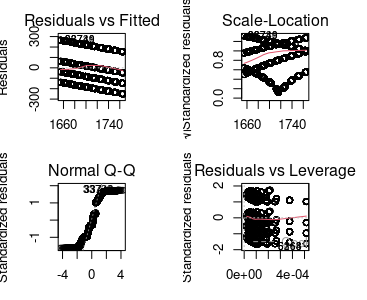
\includegraphics[width=0.60\textwidth]{imagenes/Rplot07.png}
    \caption{Gráficas diagnósticas del modelo ANOVA}
    \label{fig:suposiciones}
\end{figure}

\subsection{Segmentación de los datos}

Se ha realizado una segmentación de los registros del primer dataset en función de la calificación obtenida por los grupos que han realizado las acciones en los mapas.

Para ello, se ha sustituido la columna \emph{Team} del segundo dataset por el nombre del grupo en cada caso y se ha eliminado la columna \emph{Group}. Después de realizar este proceso el dataset tiene la forma que se muestra en la Tabla \ref{table:8}

% Segundo dataset tras cambiar el contenido de la columna Team
% latex table generated in R 4.2.2 by xtable 1.8-4 package
% Sun Feb  5 13:39:47 2023
\begin{table}[ht]
\centering
\begin{tabular}{rllll}
  \hline
 & group & size & year & grade \\ 
  \hline
1 & Lesath & 4 & 1819 & 10,00 \\ 
  2 & Jabbah & 4 & 1920 & 4,01 \\ 
  3 & Haldus & 4 & 1819 & 7,96 \\ 
  4 & Elnath & 4 & 1920 & 8,95 \\ 
  5 & Keid & 4 & 1920 & 4,51 \\ 
  6 & Furud & 6 & 1415 & 7,20 \\ 
   \hline
\end{tabular}
\caption{Dataset 2 tras ser preparado para hacer join}
\label{table:8}
\end{table}

A continuación, se transformarán los valores de la columna \emph{grade} a tipo \texttt{double} y se agruparán los datos de este dataset por grupo y año, calculando la calificación media de las prácticas para cada par grupo-año. El resultado de realizar esta operación puede apreciarse ne la Tabla \ref{table:9}.

% Agrupación del segundo dataset por grupo y año
% latex table generated in R 4.2.2 by xtable 1.8-4 package
% Sun Feb  5 13:46:44 2023
\begin{table}[ht]
\centering
\begin{tabular}{rllll}
  \hline
 & group & year & size & mean\_grade \\ 
  \hline
1 & Achernar & 1314 & 6 &  9.40 \\ 
  2 & Achernar & 1415 & 5 &  9.00 \\ 
  3 & Achernar & 1516 & 5 &  8.20 \\ 
  4 & Achernar & 1617 & 5 & 10.00 \\ 
  5 & Achernar & 1718 & 5 &  8.33 \\ 
  6 & Bellatrix & 1516 & 5 &  8.20 \\ 
   \hline
\end{tabular}
\caption{Dataset 2 tras agrupar por grupo y año}
\label{table:9}
\end{table}

Ahora, se juntan ambos datasets usando la función \texttt{inner\_join} por grupo y año. El resultado de esta operación puede observarse en la Tabla \ref{table:10}.

% inner_join de los dos datasets
% latex table generated in R 4.2.2 by xtable 1.8-4 package
% Sun Feb  5 13:50:57 2023
\begin{table}[ht]
\centering
\begin{tabular}{rlllllll}
  \hline
 & group & year & size & mean\_grade & date & map & action \\ 
  \hline
1 & Achernar & 1516 & 5 & 8.2 & 17/10/2015 19:41:45 & 0 & 0 \\ 
  2 & Achernar & 1516 & 5 & 8.2 & 22/10/2015 17:29:21 & 1 & 1 \\ 
  3 & Achernar & 1516 & 5 & 8.2 & 22/10/2015 17:29:22 & 1 & 2 \\ 
  4 & Achernar & 1516 & 5 & 8.2 & 22/10/2015 17:29:39 & 1 & 3 \\ 
  5 & Achernar & 1516 & 5 & 8.2 & 22/10/2015 17:34:09 & 1 & 1 \\ 
  6 & Achernar & 1516 & 5 & 8.2 & 22/10/2015 17:34:10 & 1 & 2 \\ 
   \hline
\end{tabular}
\caption{Unión de ambos datasets}
\label{table:10}
\end{table}

Por último, se separarán los datos de esta última tabla en función de las calificaciones obtenidas por los diferentes grupos:
\begin{itemize}
	\item \textbf{Suspenso:} calificación mayor o igual que $0$ y menor que $5$.
	\item \textbf{Aprobado:} calificación mayor o igual que $5$ y menor que $7$.
	\item \textbf{Notable:} calificación mayor o igual que $7$ y menor que $9$.
	\item \textbf{Sobresaliente:} calificación mayor o igual qye $9$ y menor que $10$.
	\item \textbf{Matrícula de Honor:} calificación igual a $10$.
\end{itemize}

Una muestra de los datasets generados tras la segmentación puede apreciarse en las tablas \ref{table:11}, \ref{table:12}, \ref{table:13}, \ref{table:14} y \ref{table:15}.

% latex table generated in R 4.2.2 by xtable 1.8-4 package
% Sun Feb  5 18:45:16 2023
\begin{table}[ht]
\centering
\begin{tabular}{rlllllll}
  \hline
 & group & year & size & mean\_grade & date & map & action \\ 
  \hline
1 & Girtab & 1617 & 6 & 4.67 & 15/11/2016 7:31:31  & 1 & 1 \\ 
  2 & Girtab & 1617 & 6 & 4.67 & 15/11/2016 7:31:53  & 1 & 1 \\ 
  3 & Girtab & 1617 & 6 & 4.67 & 15/11/2016 12:50:03 & 1 & 1 \\ 
  4 & Girtab & 1617 & 6 & 4.67 & 15/11/2016 12:50:28 & 1 & 1 \\ 
  5 & Girtab & 1617 & 6 & 4.67 & 15/11/2016 13:27:27 & 1 & 1 \\ 
  6 & Girtab & 1617 & 6 & 4.67 & 15/11/2016 13:27:58 & 1 & 1 \\ 
   \hline
\end{tabular}
\caption{Muestra del dataset de los grupos \textbf{suspensos}. Consta de $2397$ registros con $7$ campos cada uno.}
\label{table:11}
\end{table}

% latex table generated in R 4.2.2 by xtable 1.8-4 package
% Sun Feb  5 18:47:50 2023
\begin{table}[ht]
\centering
\begin{tabular}{rlllllll}
  \hline
 & group & year & size & mean\_grade & date & map & action \\ 
  \hline
1 & Bellatrix & 1920 & 4 & 6.835 & 05/11/2019 10:24:51 & 1 & 1 \\ 
  2 & Bellatrix & 1920 & 4 & 6.835 & 05/11/2019 10:24:51 & 1 & 2 \\ 
  3 & Bellatrix & 1920 & 4 & 6.835 & 05/11/2019 10:25:04 & 1 & 1 \\ 
  4 & Bellatrix & 1920 & 4 & 6.835 & 05/11/2019 10:25:26 & 1 & 2 \\ 
  5 & Bellatrix & 1920 & 4 & 6.835 & 05/11/2019 10:25:39 & 1 & 1 \\ 
  6 & Bellatrix & 1920 & 4 & 6.835 & 05/11/2019 10:25:45 & 1 & 2 \\ 
   \hline
\end{tabular}
\caption{Muestra del dataset de los grupos \textbf{aprobados}. Consta de $7053$ registros con $7$ campos cada uno.}
\label{table:12}
\end{table}

% latex table generated in R 4.2.2 by xtable 1.8-4 package
% Sun Feb  5 18:50:12 2023
\begin{table}[ht]
\centering
\begin{tabular}{rlllllll}
  \hline
 & group & year & size & mean\_grade & date & map & action \\ 
  \hline
1 & Achernar & 1516 & 5 & 8.2 & 17/10/2015 19:41:45 & 0 & 0 \\ 
  2 & Achernar & 1516 & 5 & 8.2 & 22/10/2015 17:29:21 & 1 & 1 \\ 
  3 & Achernar & 1516 & 5 & 8.2 & 22/10/2015 17:29:22 & 1 & 2 \\ 
  4 & Achernar & 1516 & 5 & 8.2 & 22/10/2015 17:29:39 & 1 & 3 \\ 
  5 & Achernar & 1516 & 5 & 8.2 & 22/10/2015 17:34:09 & 1 & 1 \\ 
  6 & Achernar & 1516 & 5 & 8.2 & 22/10/2015 17:34:10 & 1 & 2 \\ 
   \hline
\end{tabular}
\caption{Muestra del dataset de los grupos con \textbf{notable}. Consta de $18840$ registros con $7$ campos cada uno.}
\label{table:13}
\end{table}

% latex table generated in R 4.2.2 by xtable 1.8-4 package
% Sun Feb  5 18:51:55 2023
\begin{table}[ht]
\centering
\begin{tabular}{rlllllll}
  \hline
 & group & year & size & mean\_grade & date & map & action \\ 
  \hline
1 & Bellatrix & 1617 & 5 & 9.72 & 07/11/2016 11:13:31 & 1 & 1 \\ 
  2 & Bellatrix & 1617 & 5 & 9.72 & 07/11/2016 11:36:59 & 1 & 1 \\ 
  3 & Bellatrix & 1617 & 5 & 9.72 & 07/11/2016 11:41:07 & 1 & 1 \\ 
  4 & Bellatrix & 1617 & 5 & 9.72 & 07/11/2016 11:42:22 & 1 & 1 \\ 
  5 & Bellatrix & 1617 & 5 & 9.72 & 07/11/2016 11:45:37 & 1 & 1 \\ 
  6 & Bellatrix & 1617 & 5 & 9.72 & 07/11/2016 11:49:23 & 1 & 1 \\ 
   \hline
\end{tabular}
\caption{Muestra del dataset de los grupos con \textbf{sobresaliente}. Consta de $17891$ registros con $7$ campos cada uno.}
\label{table:14}
\end{table}

% latex table generated in R 4.2.2 by xtable 1.8-4 package
% Sun Feb  5 18:53:13 2023
\begin{table}[ht]
\centering
\begin{tabular}{rlllllll}
  \hline
 & group & year & size & mean\_grade & date & map & action \\ 
  \hline
1 & Achernar & 1617 & 5 & 10 & 09/11/2016 21:23:22 & 1 & 1 \\ 
  2 & Achernar & 1617 & 5 & 10 & 09/11/2016 21:25:11 & 1 & 1 \\ 
  3 & Achernar & 1617 & 5 & 10 & 10/11/2016 0:21:37  & 1 & 1 \\ 
  4 & Achernar & 1617 & 5 & 10 & 10/11/2016 0:22:50  & 1 & 1 \\ 
  5 & Achernar & 1617 & 5 & 10 & 10/11/2016 0:23:12  & 1 & 1 \\ 
  6 & Achernar & 1617 & 5 & 10 & 10/11/2016 0:25:53  & 1 & 1 \\ 
   \hline
\end{tabular}
\caption{Muestra del dataset de los grupos con \textbf{matrícula de honor}. Consta de $1646$ registros con $7$ campos cada uno.}
\label{table:15}
\end{table}

\section{Extracción de procesos ocultos en los datasets}
\subsection{Extracción de los procesos con DISCO}

\begin{figure}[H]
    \centering
    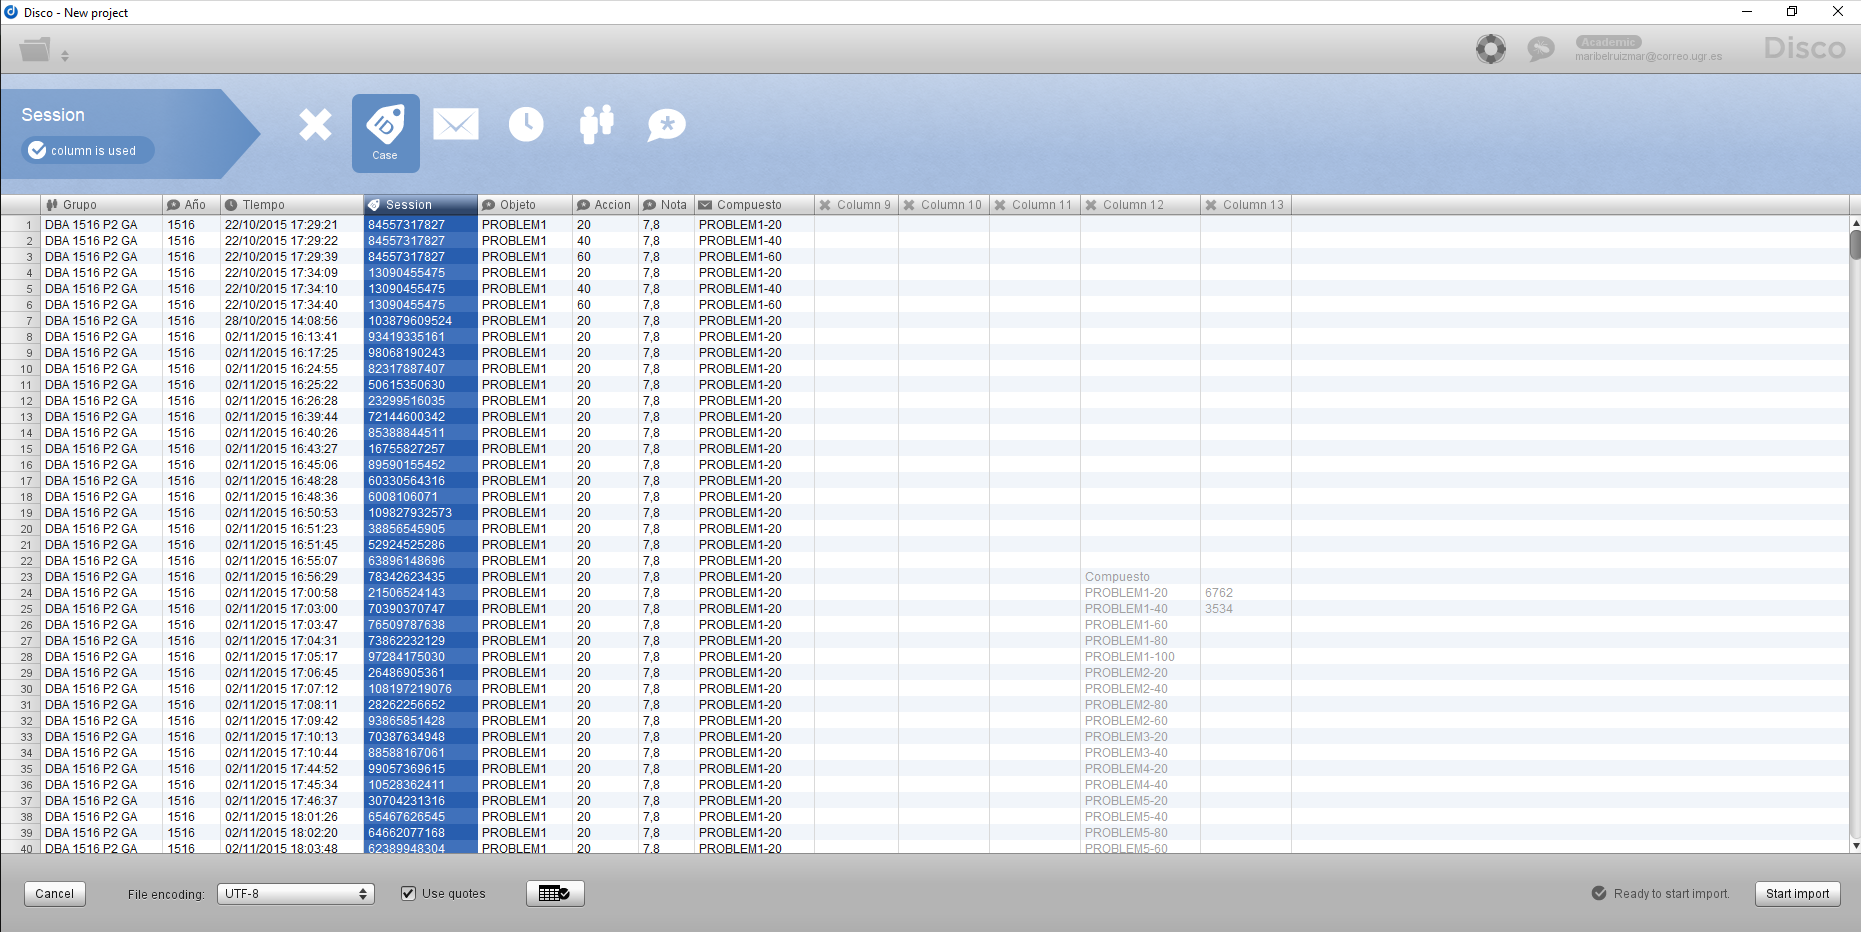
\includegraphics[width=1.25\textwidth]{imagenes/DISCO_compound/DISCO.png}
    \caption{Análisis de procesos del dataset compuesto (acción mapa).}
    \label{fig:DISCO}
\end{figure}

\begin{figure}[H]
    \centering
    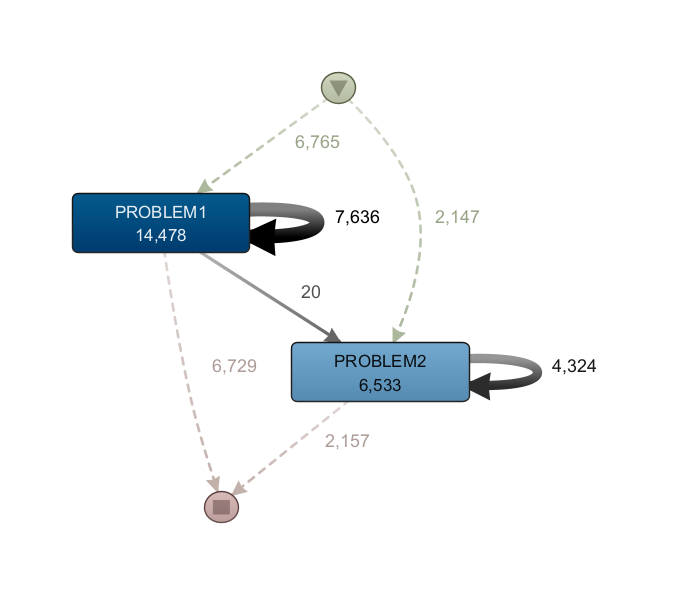
\includegraphics[width=0.75\textwidth]{imagenes/DISCO_map/Dataset Fusionado.png}
    \caption{Análisis de procesos del dataset compuesto (acción mapa).}
    \label{fig:datasetFusionado}
\end{figure}

\begin{figure}[H]
    \centering
    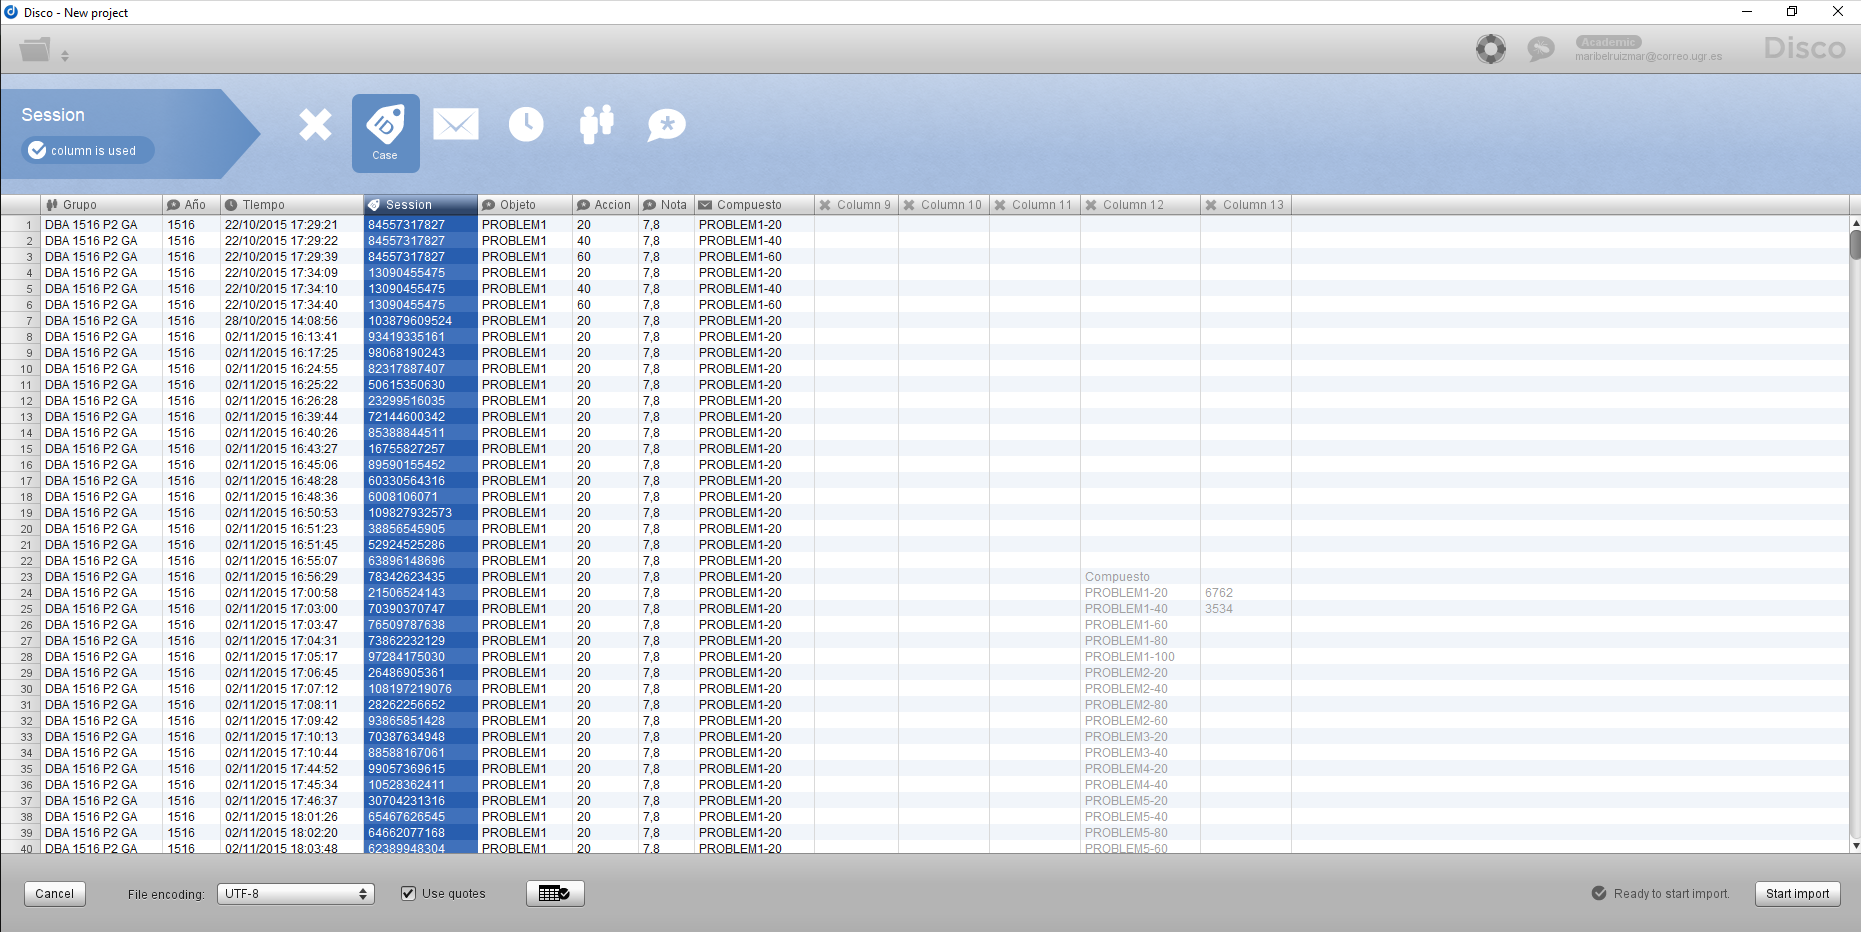
\includegraphics[width=1.25\textwidth]{imagenes/DISCO_compound/DISCO.png}
    \caption{Análisis de procesos del dataset compuesto (acción compuesta).}
    \label{fig:DISCO}
\end{figure}

\begin{figure}[H]
    \centering
    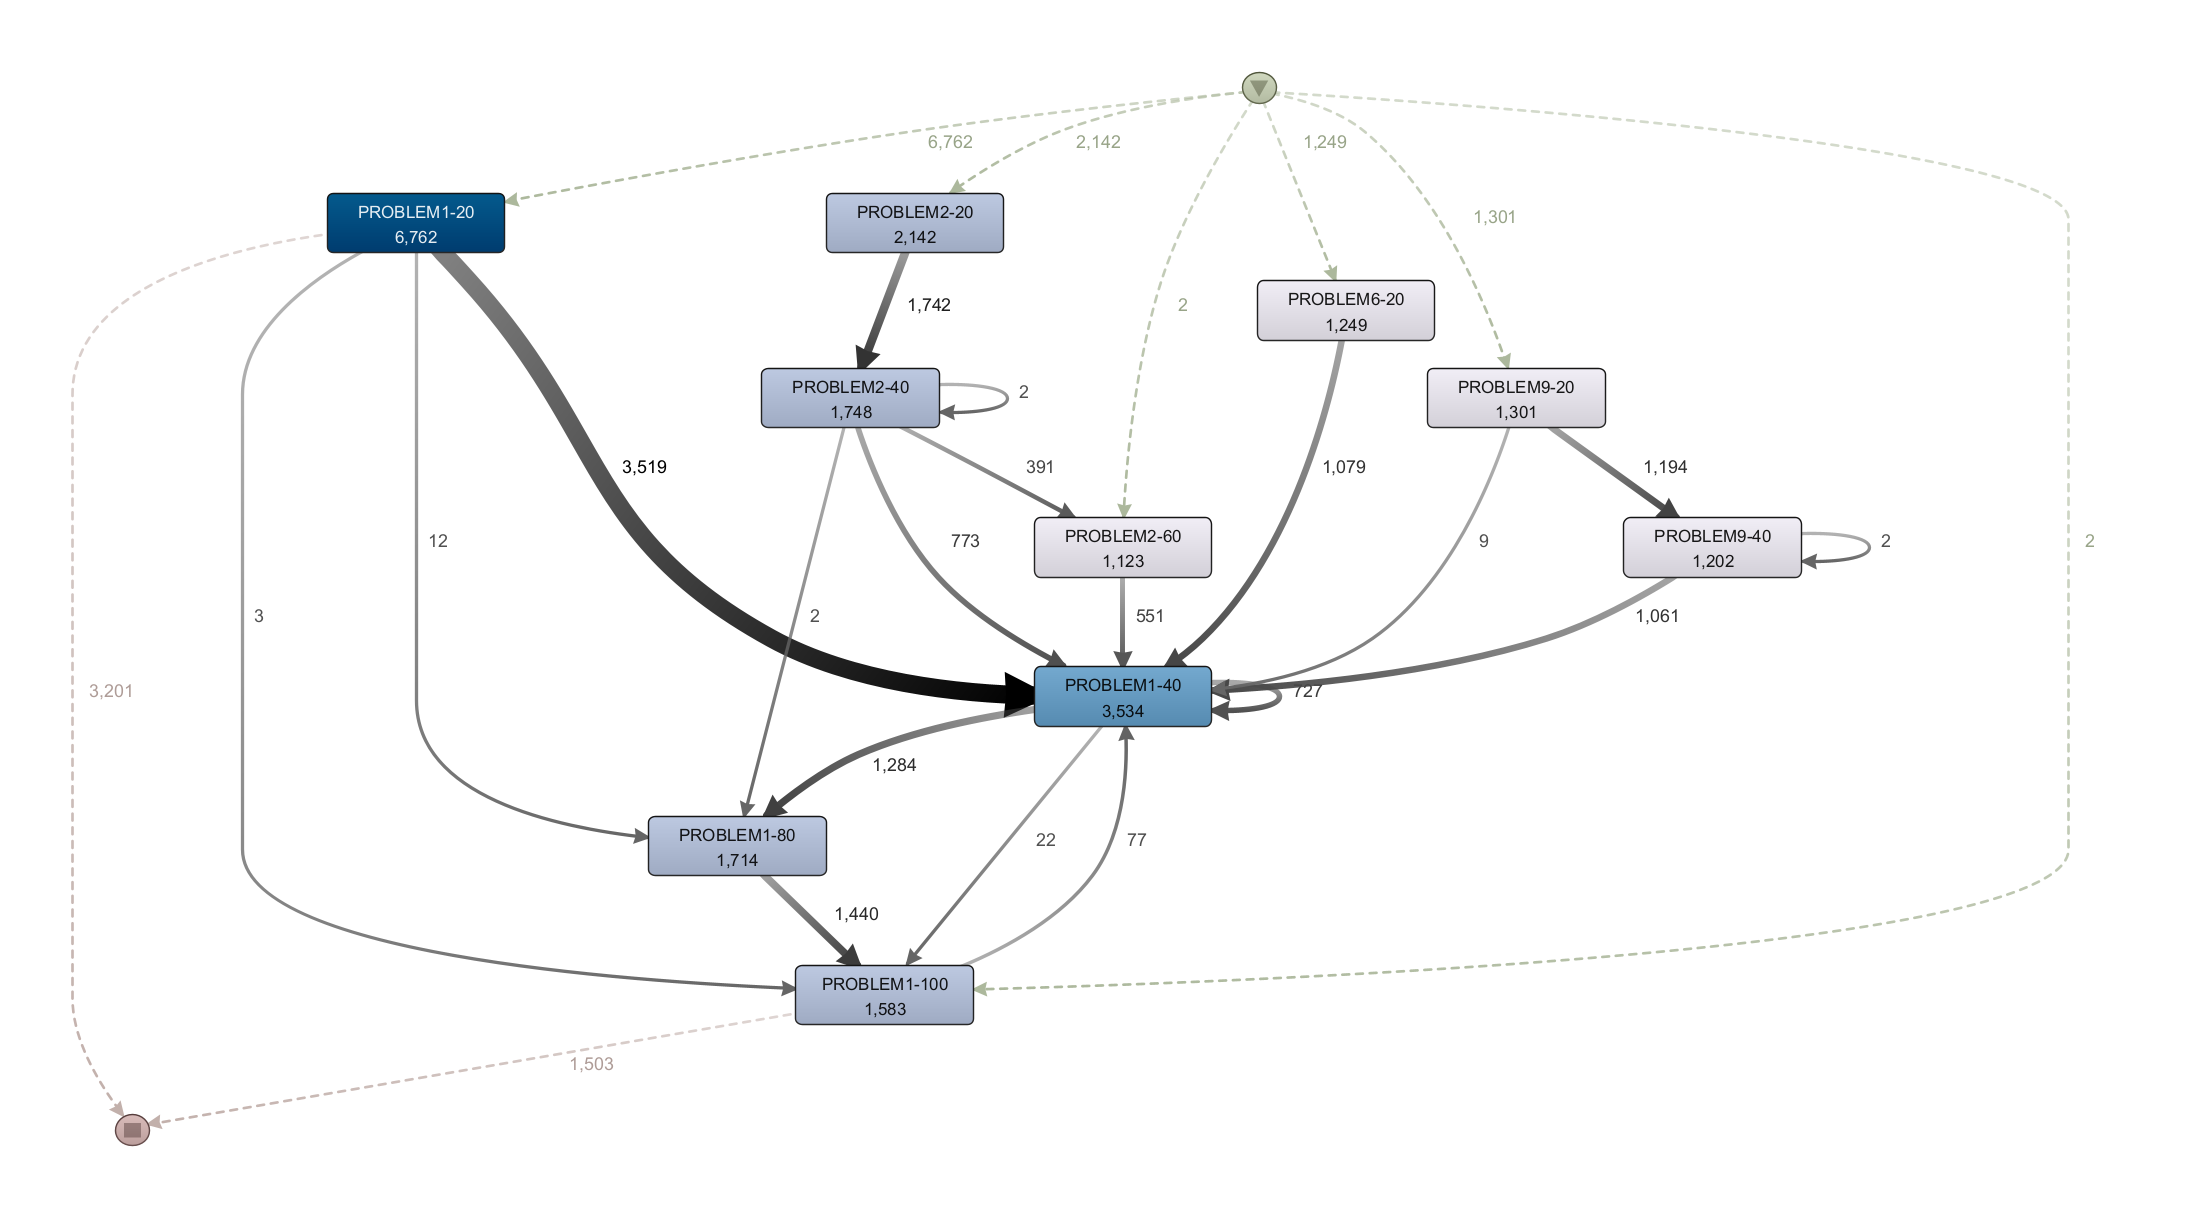
\includegraphics[width=1.25\textwidth]{imagenes/DISCO_compound/Dataset Fusionado - Compuesto.png}
    \caption{Análisis de procesos del dataset compuesto (acción compuesta).}
    \label{fig:datasetFusionadoCompuesto}
\end{figure}

\subsection{Segmentación por años}

\begin{figure}[H]
  \begin{subfigure}[t]{0.60\textwidth}
    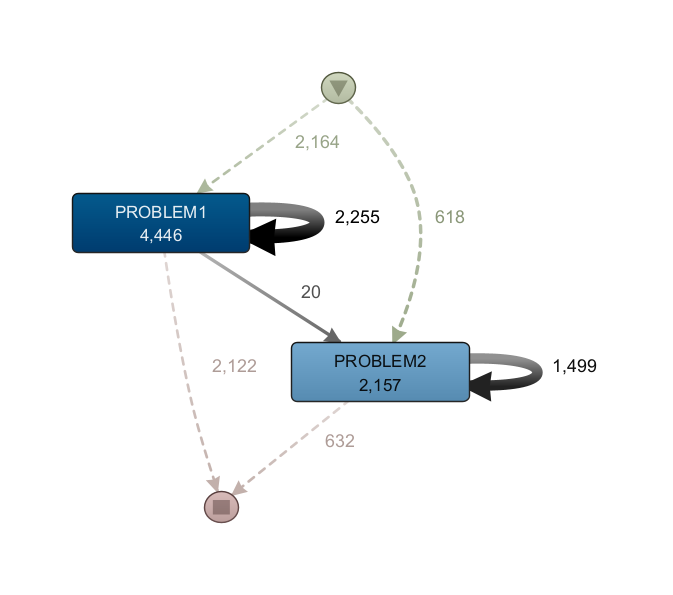
\includegraphics[width=1.10\textwidth, height=1.10\textwidth]{imagenes/DISCO_map/Dataset FusionadoYear1516.png}
    \caption{Extracción de procesos del curso académico 1516 (acción mapa).}
    \label{fig:mapAño1516}
  \end{subfigure}
  \hfill
  \begin{subfigure}[t]{0.60\textwidth}
    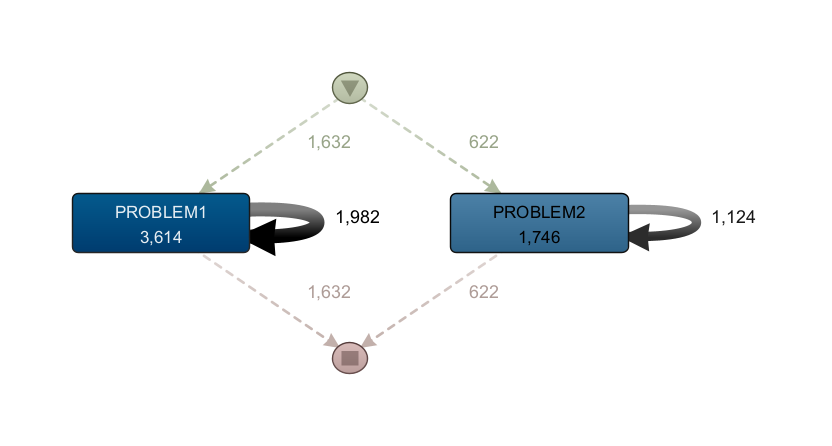
\includegraphics[width=1.10\textwidth, height=0.80\textwidth]{imagenes/DISCO_map/Dataset FusionadoYear1617.png}
    \caption{Extracción de procesos del curso académico 1617 (acción mapa).}
    \label{fig:mapAño1617}
  \end{subfigure}
  \hfill
  \begin{subfigure}[t]{0.60\textwidth}
    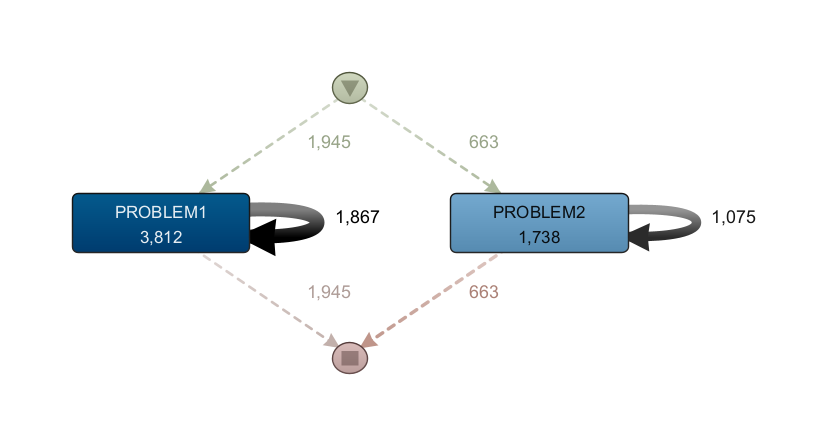
\includegraphics[width=1.10\textwidth, height=0.80\textwidth]{imagenes/DISCO_map/Dataset FusionadoYear1718.png}
    \caption{Extracción de procesos del curso académico 1718 (acción mapa).}
    \label{fig:mapAño1718}
  \end{subfigure}
  \hfill
  \begin{subfigure}[t]{0.60\textwidth}
    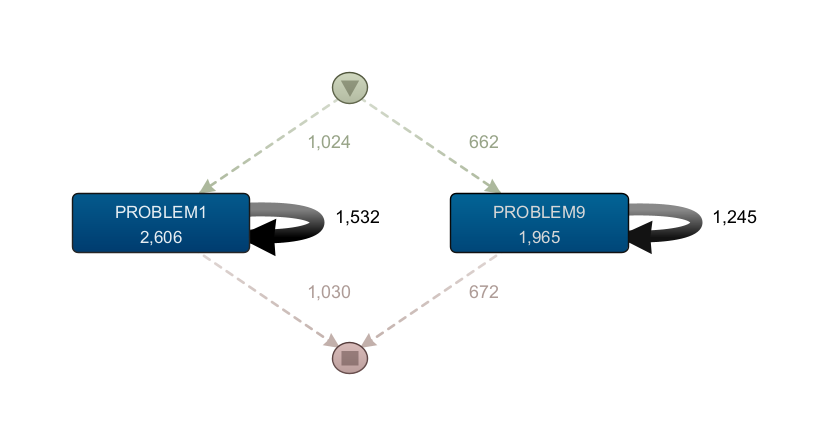
\includegraphics[width=1.10\textwidth, height=0.80\textwidth]{imagenes/DISCO_map/Dataset FusionadoYear1920.png}
    \caption{Extracción de procesos del curso académico 1920 (acción mapa).}
    \label{fig:mapAño1920}
  \end{subfigure}
  \caption{Extracción de procesos de los diferentes cursos académicos (acción mapa/problema).}
\end{figure}

\begin{figure}[H]
    \centering
    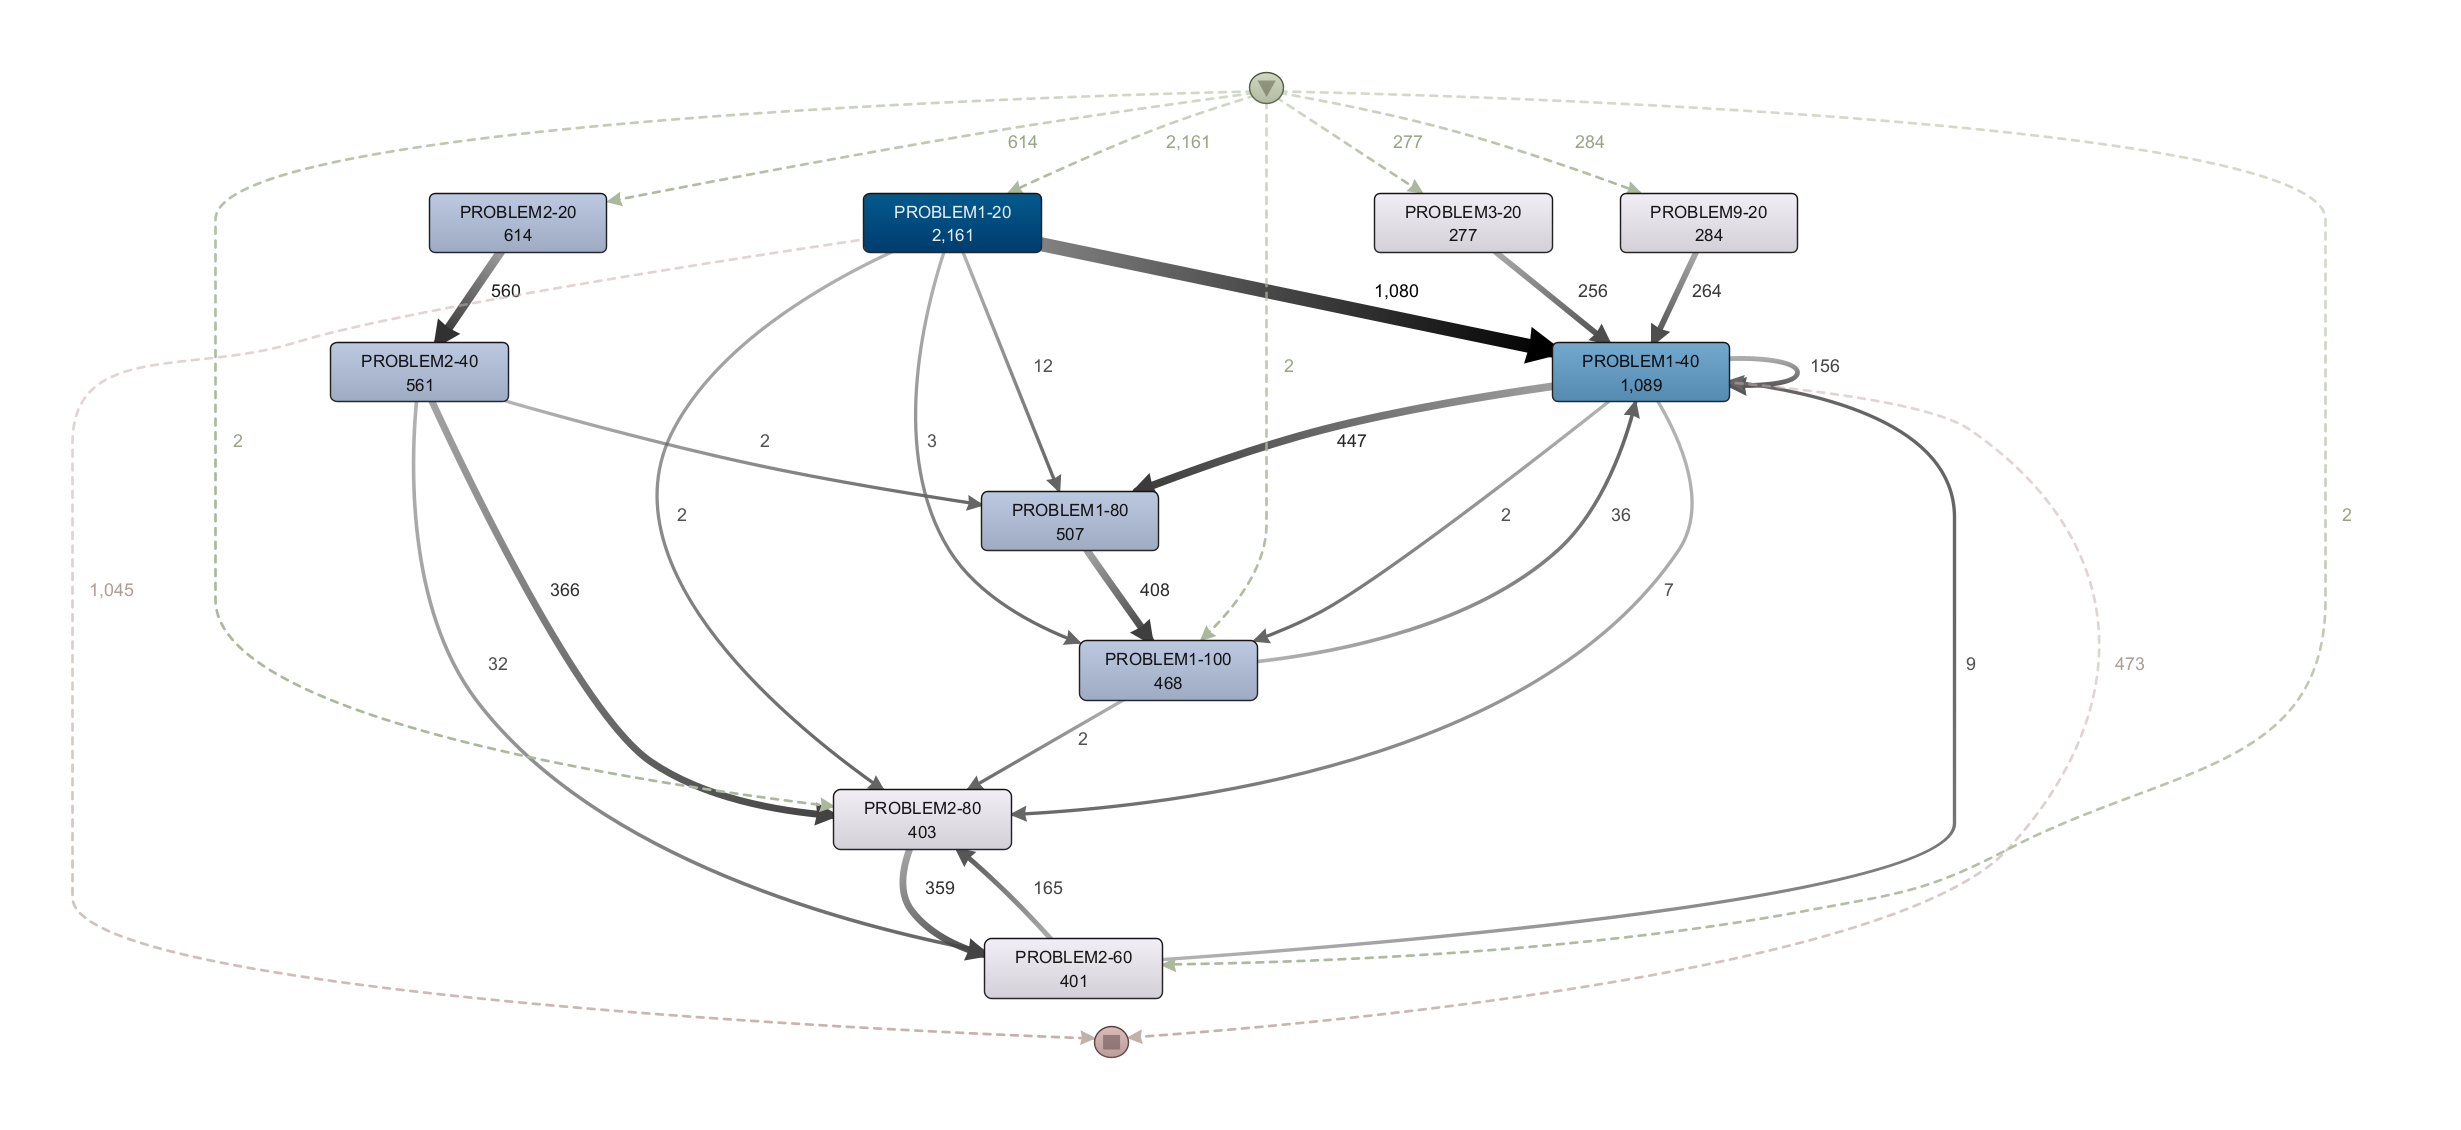
\includegraphics[width=1.25\textwidth]{imagenes/DISCO_compound/Year1516.png}
    \caption{Extracción de procesos del curso académico 1516 (acción compuesta).}
    \label{fig:año1516}
\end{figure}

\begin{figure}[H]
    \centering
    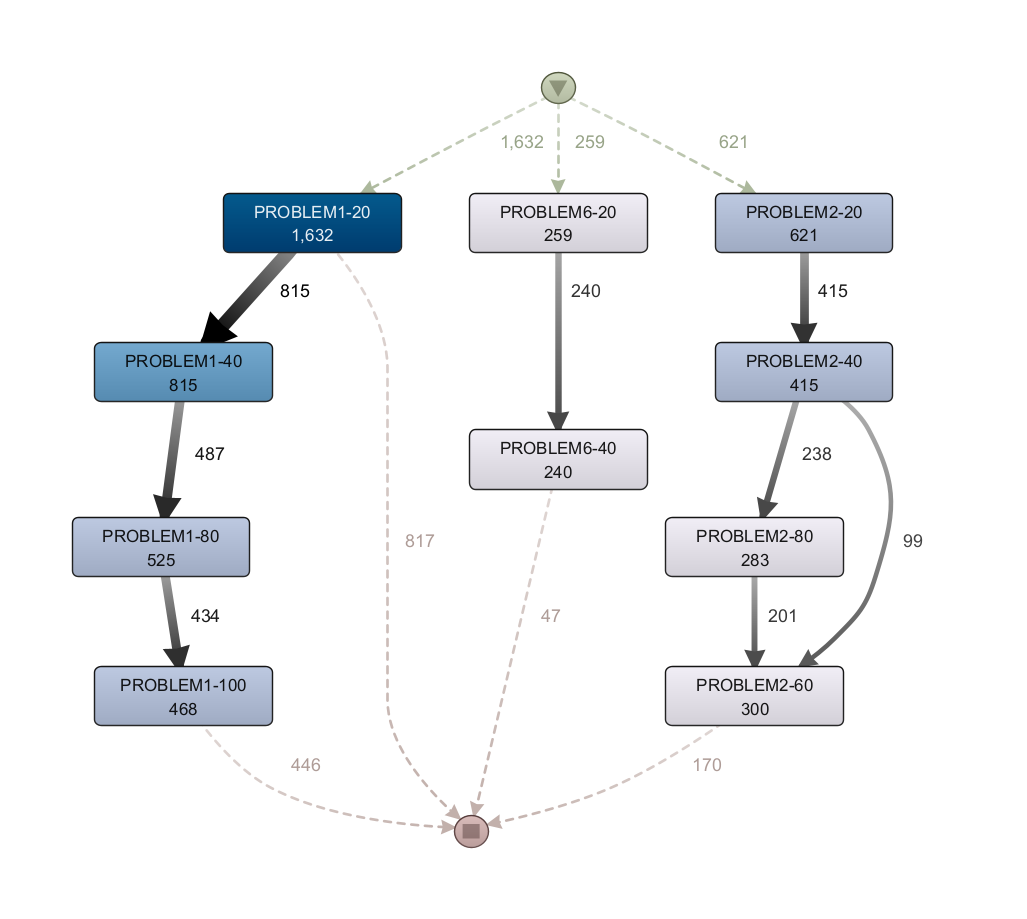
\includegraphics[width=1.25\textwidth]{imagenes/DISCO_compound/Year1617.png}
    \caption{Extracción de procesos del curso académico 1617 (acción compuesta).}
    \label{fig:año1617}
\end{figure}

\begin{figure}[H]
    \centering
    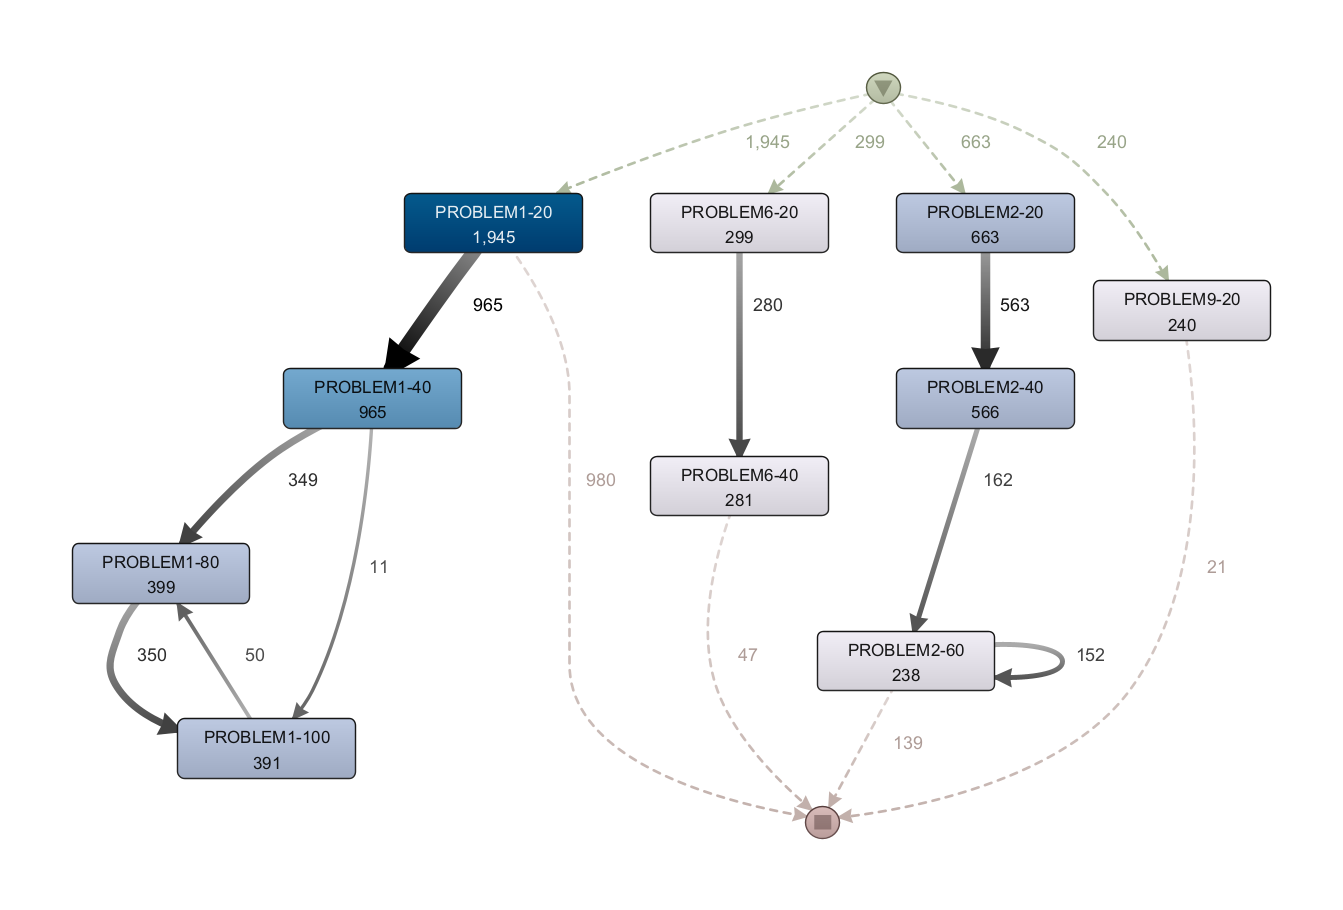
\includegraphics[width=1.25\textwidth]{imagenes/DISCO_compound/Year1718.png}
    \caption{Extracción de procesos del curso académico 1718 (acción compuesta).}
    \label{fig:año1718}
\end{figure}

\begin{figure}[H]
    \centering
    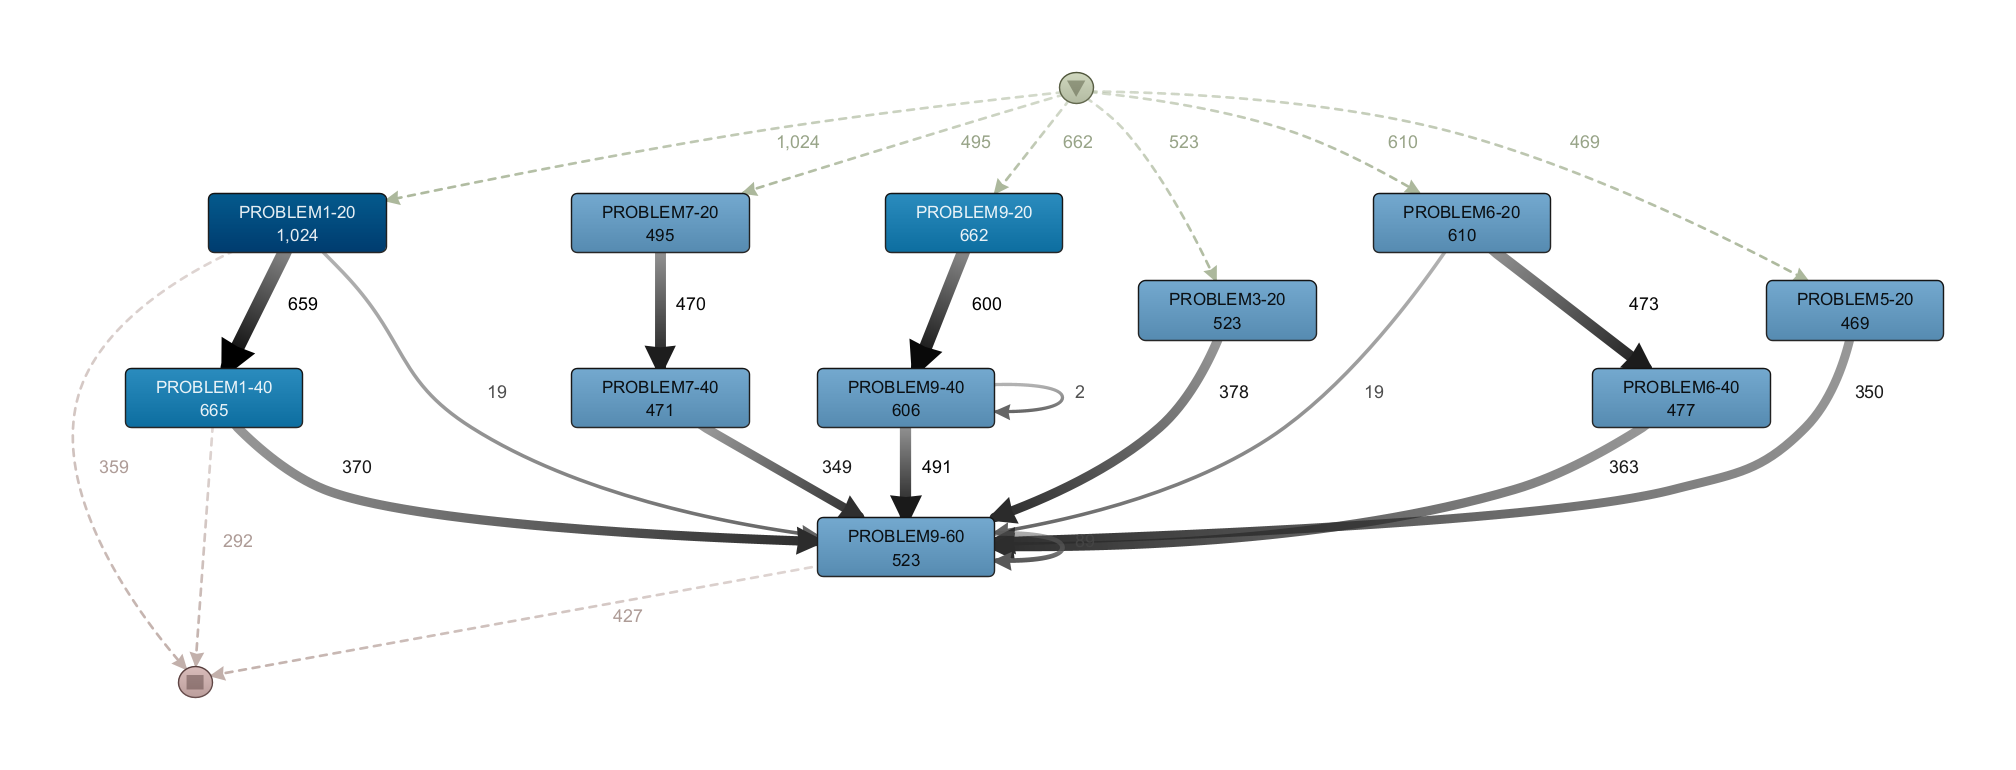
\includegraphics[width=1.25\textwidth]{imagenes/DISCO_compound/Year1920.png}
    \caption{Extracción de procesos del curso académico 1920 (acción compuesta).}
    \label{fig:año1920}
\end{figure}

\subsection{Segmentación por calificaciones}

De ahora en adelante se considerará que la calificación de un grupo es \emph{``baja''} si es inferior a $7.5$, \emph{``media-baja''} si es igual o mayor que $7.5$ y menor a $8.5$, \emph{``media-alta''} si es igual a o mayor que $8.5$ e inferior a $9.5$ y \emph{``alta''} si es igual o superior a $9.5$.

\begin{figure}[H]
  \begin{subfigure}[t]{0.60\textwidth}
    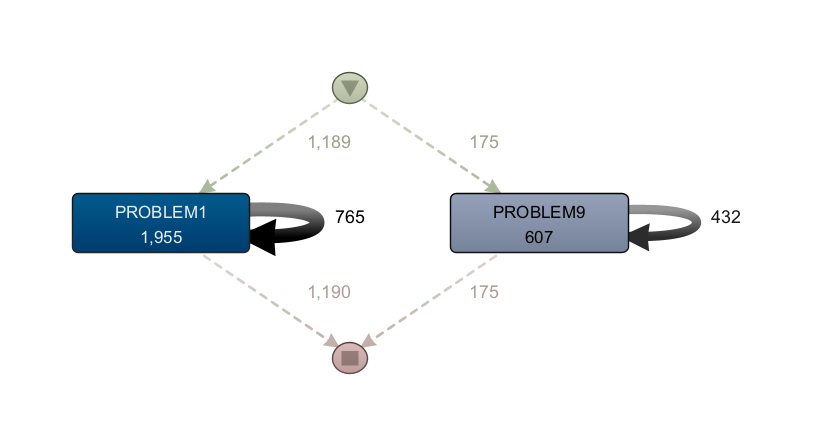
\includegraphics[width=1.10\textwidth, height=0.80\textwidth]{imagenes/DISCO_map/Dataset FusionadoWorstGrades.png}
    \caption{Extracción de procesos del dataset integrado por las acciones mapa de los grupos con calificación \emph{``baja''}.}
    \label{fig:mapWorstGrades}
  \end{subfigure}
  \hfill
  \begin{subfigure}[t]{0.60\textwidth}
    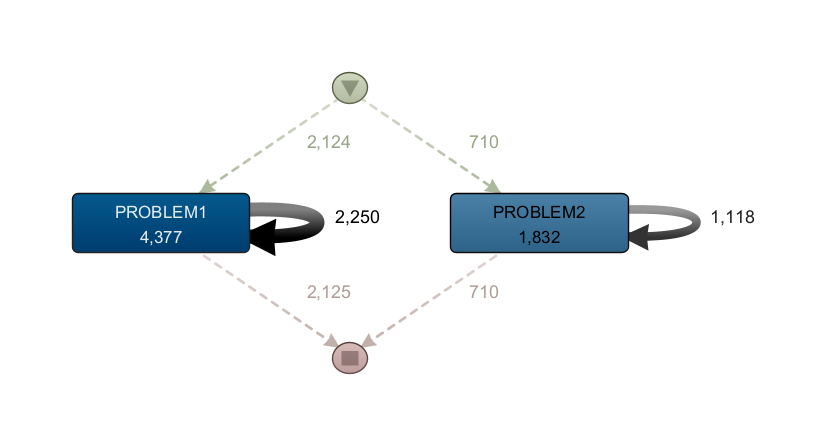
\includegraphics[width=1.10\textwidth, height=0.80\textwidth]{imagenes/DISCO_map/Dataset FusionadoMidLowGrades.png}
    \caption{Extracción de procesos del dataset integrado por las acciones mapa de los grupos con calificación \emph{``media-baja''}.}
    \label{fig:mapMidLowGrades}
  \end{subfigure}
  \hfill
  \begin{subfigure}[t]{0.60\textwidth}
    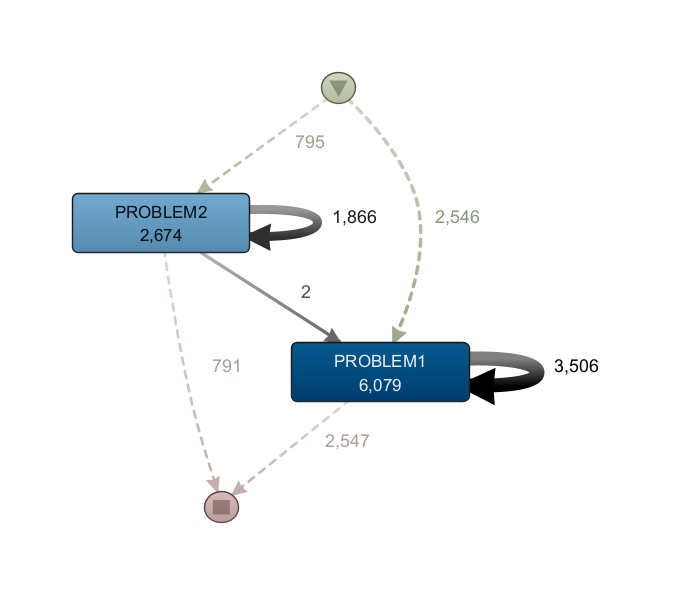
\includegraphics[width=1.10\textwidth, height=1.10\textwidth]{imagenes/DISCO_map/Dataset FusionadoMidHighGrades.png}
    \caption{Extracción de procesos del dataset integrado por las acciones mapa de los grupos con calificación \emph{``media-alta''}.}
    \label{fig:mapMidHighGrades}
  \end{subfigure}
  \hfill
  \begin{subfigure}[t]{0.60\textwidth}
    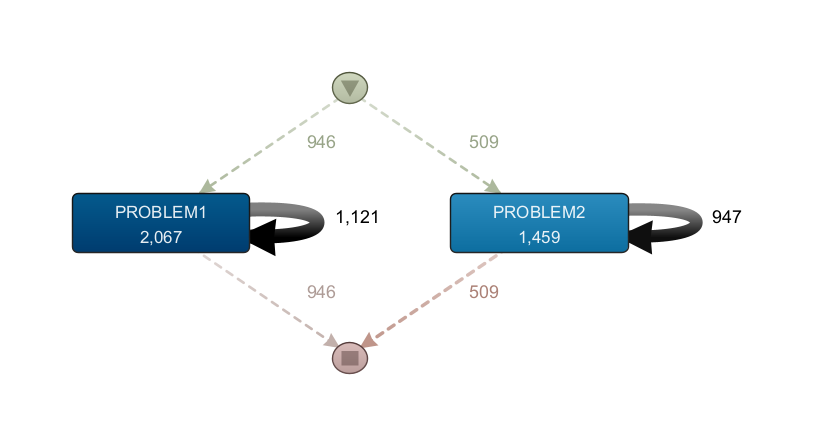
\includegraphics[width=1.10\textwidth, height=0.80\textwidth]{imagenes/DISCO_map/Dataset FusionadoHighGrades.png}
    \caption{Extracción de procesos del dataset integrado por las acciones mapa de los grupos con calificación \emph{``alta''}.}
    \label{fig:mapHighGrades}
  \end{subfigure}
  \caption{Extracción de procesos del dataset integrado por las acciones mapa de los grupos según sus calificaciones.}
\end{figure}

\begin{figure}[H]
    \centering
    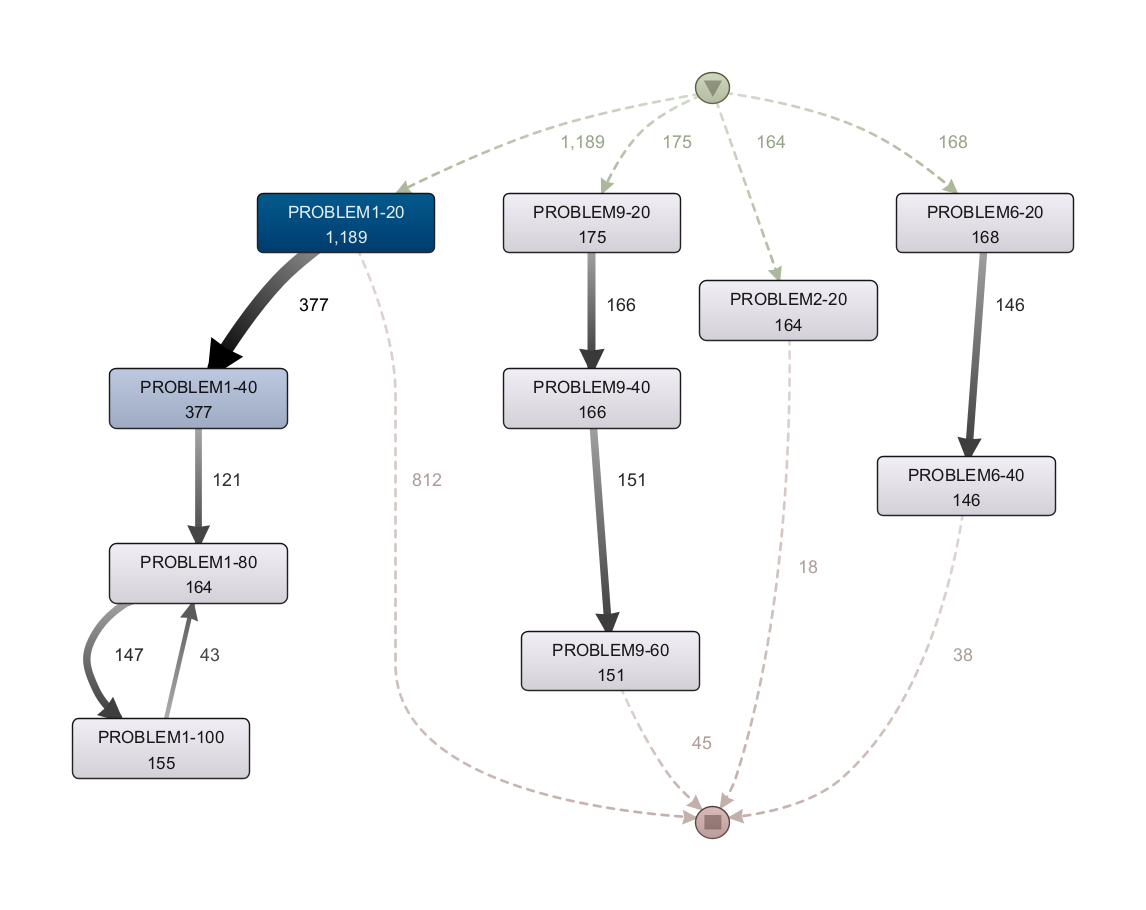
\includegraphics[width=1.25\textwidth]{imagenes/DISCO_compound/WorstGrades.png}
    \caption{Extracción de procesos del dataset integrado por las acciones compuestas de los grupos con calificación \emph{``baja''}.}
    \label{fig:worstGrades}
\end{figure}

\begin{figure}[H]
    \centering
    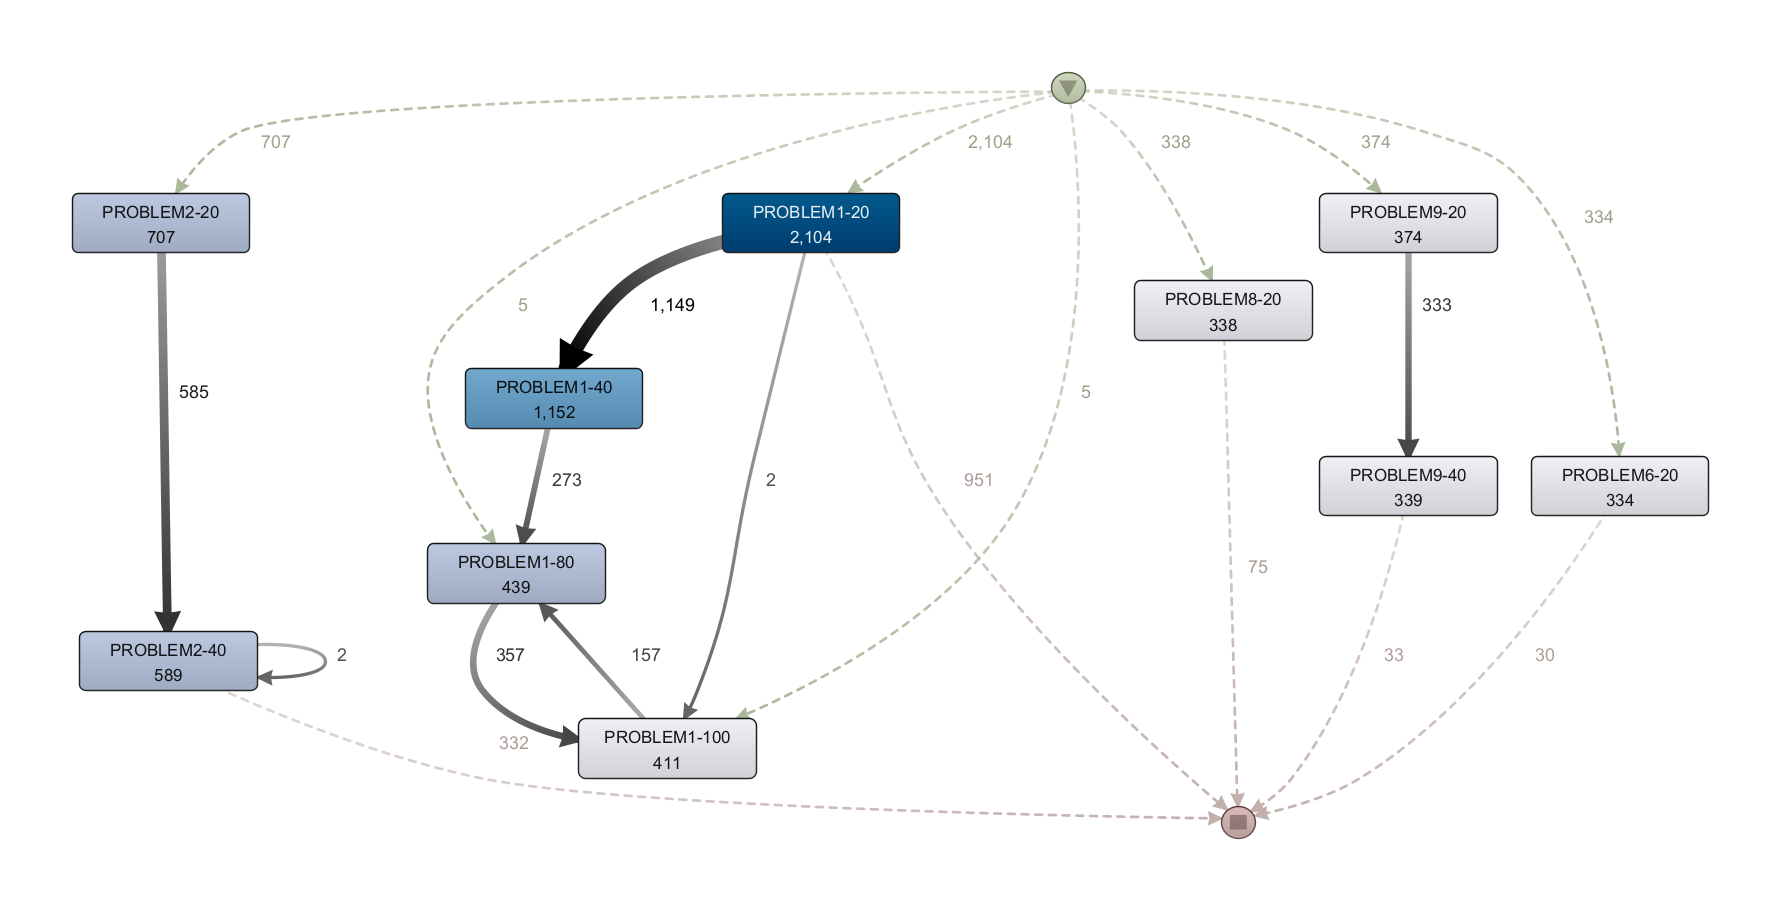
\includegraphics[width=1.25\textwidth]{imagenes/DISCO_compound/MidLowGrades.png}
    \caption{Extracción de procesos del dataset integrado por las acciones compuestas de los grupos con calificación \emph{``media-baja''}.}
    \label{fig:midLowGrades}
\end{figure}

\begin{figure}[H]
    \centering
    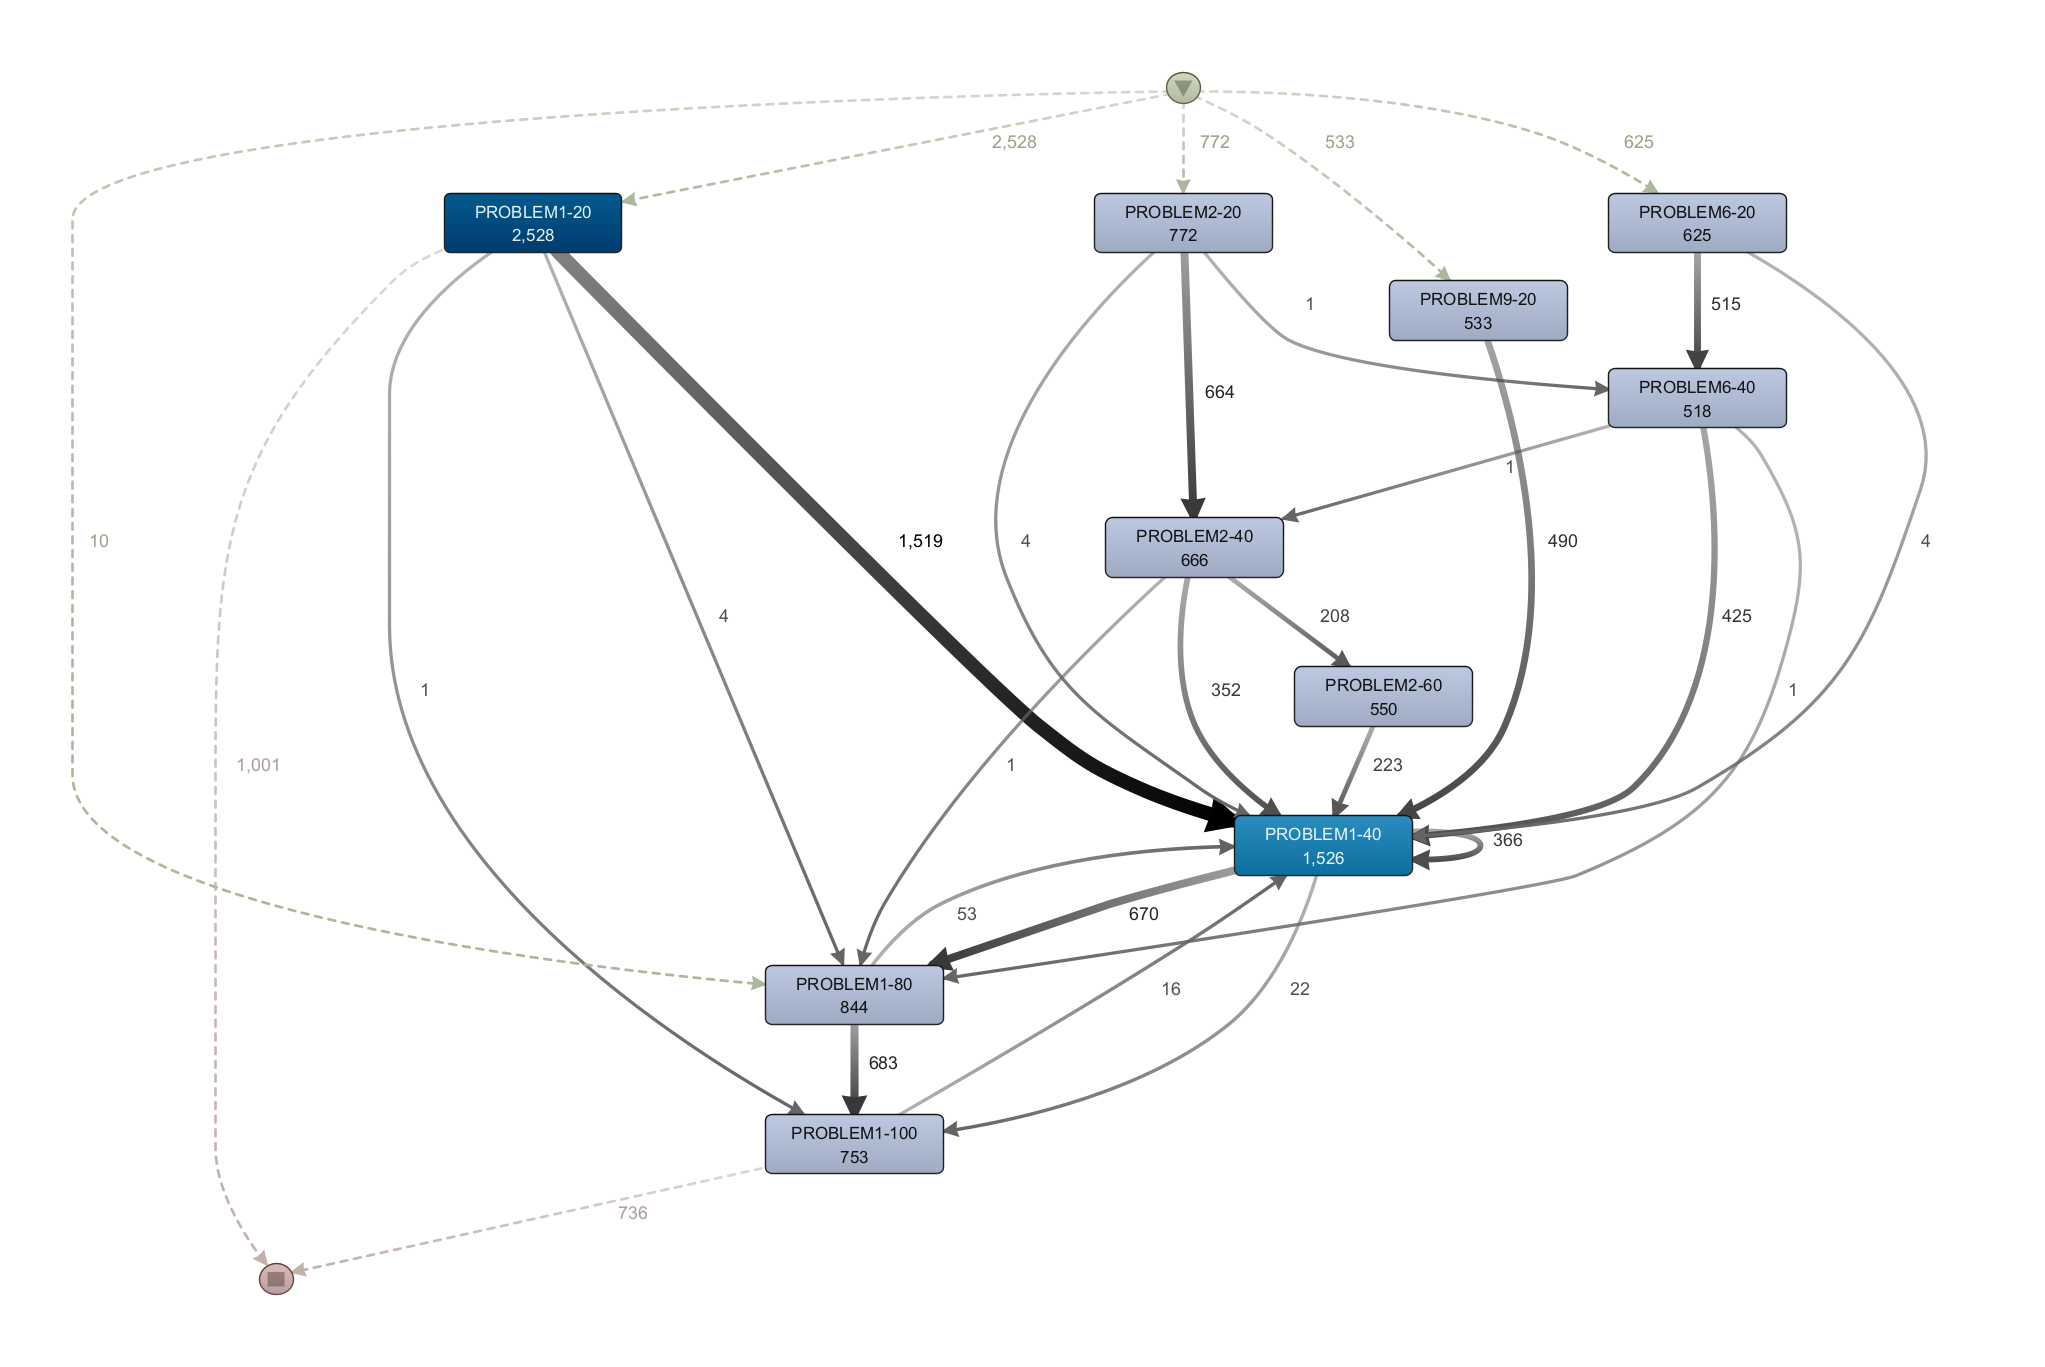
\includegraphics[width=1.25\textwidth]{imagenes/DISCO_compound/MidHighGrades.png}
    \caption{Extracción de procesos del dataset integrado por las acciones compuestas de los grupos con calificación \emph{``media-alta''}.}
    \label{fig:midHighGrades}
\end{figure}

\begin{figure}[H]
    \centering
    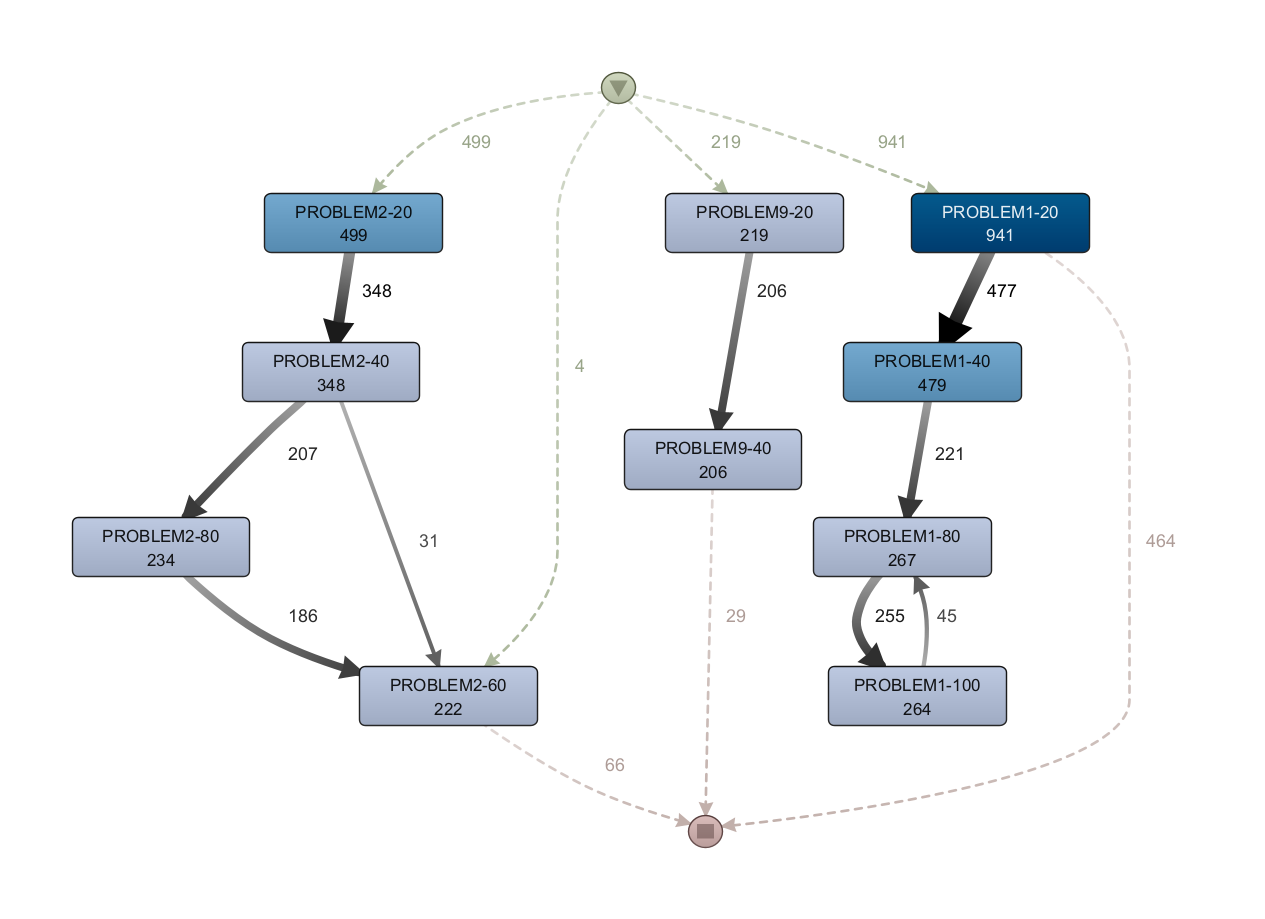
\includegraphics[width=1.25\textwidth]{imagenes/DISCO_compound/BestGrades.png}
    \caption{Extracción de procesos del dataset integrado por las acciones compuestas de los grupos con calificación \emph{``alta''}.}
    \label{fig:bestGrades}
\end{figure}


\subsection{Segmentación por año y calificación}

\begin{figure}[H]
  \begin{subfigure}[t]{0.60\textwidth}
    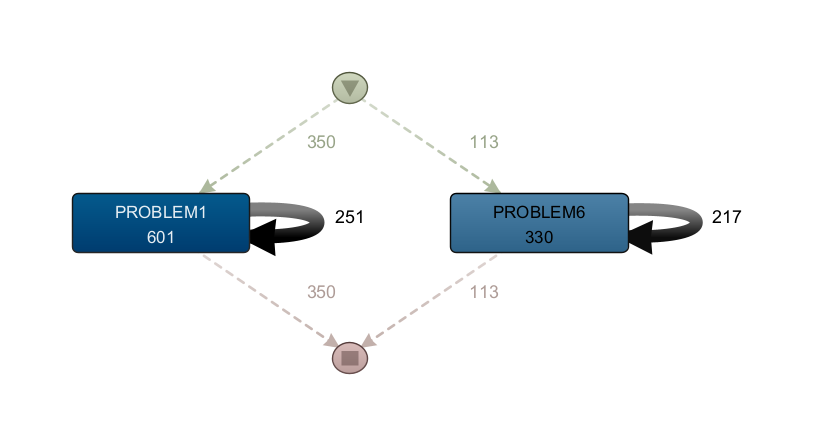
\includegraphics[width=1.10\textwidth, height=0.80\textwidth]{imagenes/DISCO_map/Dataset FusionadoYear1617WorstGrades.png}
    \caption{Extracción de procesos del dataset integrado por las acciones mapa de los grupos con calificación \emph{``baja''} del curso académico 1617.}
    \label{fig:mapYear1617WorstGrades}
  \end{subfigure}
  \hfill
  \begin{subfigure}[t]{0.60\textwidth}
    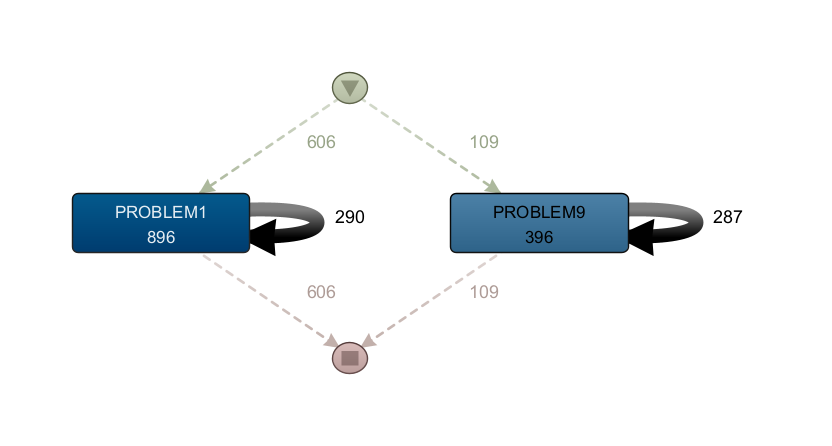
\includegraphics[width=1.10\textwidth, height=0.80\textwidth]{imagenes/DISCO_map/Dataset FusionadoYear1718WorstGrades.png}
    \caption{Extracción de procesos del dataset integrado por las acciones mapa de los grupos con calificación \emph{``baja''} del curso académico 1718.}
    \label{fig:mapYear1718WorstGrades}
  \end{subfigure}
  \hfill
  \begin{subfigure}[t]{0.60\textwidth}
    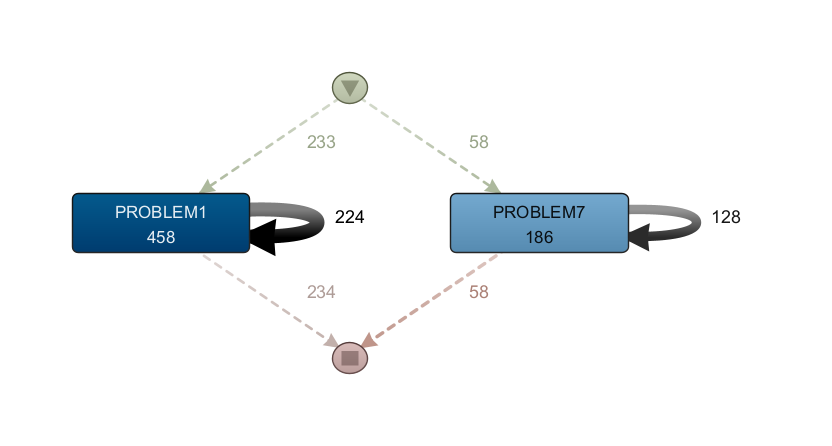
\includegraphics[width=1.10\textwidth, height=0.80\textwidth]{imagenes/DISCO_map/Dataset FusionadoYear1920WorstGrades.png}
    \caption{Extracción de procesos del dataset integrado por las acciones mapa de los grupos con calificación \emph{``baja''} del curso académico 1920.}
    \label{fig:mapYear1920WorstGrades}
  \end{subfigure}
  \caption{Extracción de procesos del dataset integrado por las acciones mapa de los grupos con calificación \emph{``baja''} a lo largo de cuatro cursos académicos.}
\end{figure}

\begin{figure}[H]
  \begin{subfigure}[t]{0.60\textwidth}
    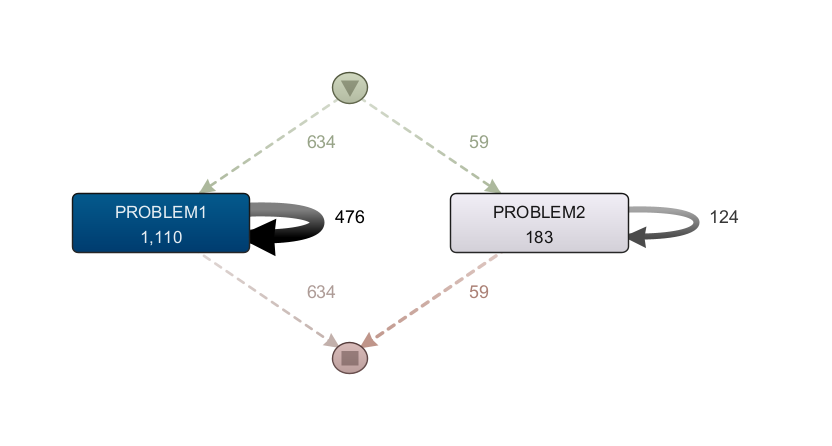
\includegraphics[width=1.10\textwidth, height=0.80\textwidth]{imagenes/DISCO_map/Dataset FusionadoYear1516MidLowGrades.png}
    \caption{Extracción de procesos del dataset integrado por las acciones mapa de los grupos con calificación \emph{``media-baja''} del curso académico 1516.}
    \label{fig:mapYear1516MidLowGrades}
  \end{subfigure}
  \hfill
  \begin{subfigure}[t]{0.60\textwidth}
    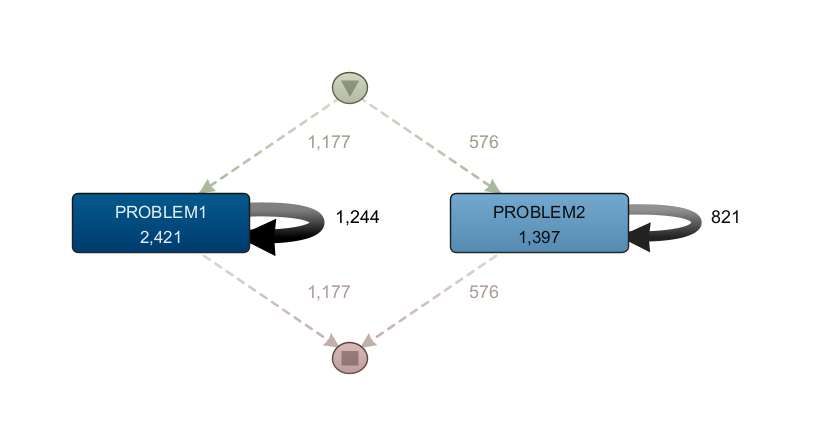
\includegraphics[width=1.10\textwidth, height=0.80\textwidth]{imagenes/DISCO_map/Dataset FusionadoYear1718MidLowGrades.png}
    \caption{Extracción de procesos del dataset integrado por las acciones mapa de los grupos con calificación \emph{``media-baja''} del curso académico 1718.}
    \label{fig:mapYear1718MidLowGrades}
  \end{subfigure}
  \hfill
  \begin{subfigure}[t]{0.60\textwidth}
    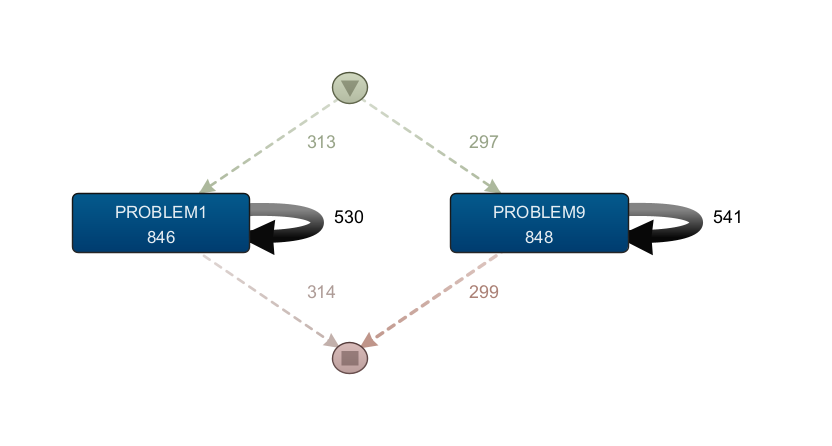
\includegraphics[width=1.10\textwidth, height=0.80\textwidth]{imagenes/DISCO_map/Dataset FusionadoYear1920MidLowGrades.png}
    \caption{Extracción de procesos del dataset integrado por las acciones mapa de los grupos con calificación \emph{``media-baja''} del curso académico 1920.}
    \label{fig:mapYear1920MidLowGrades}
  \end{subfigure}
  \caption{Extracción de procesos del dataset integrado por las acciones mapa de los grupos con calificación \emph{``media-baja''} a lo largo de cuatro cursos académicos.}
\end{figure}

\begin{figure}[H]
  \begin{subfigure}[t]{0.60\textwidth}
    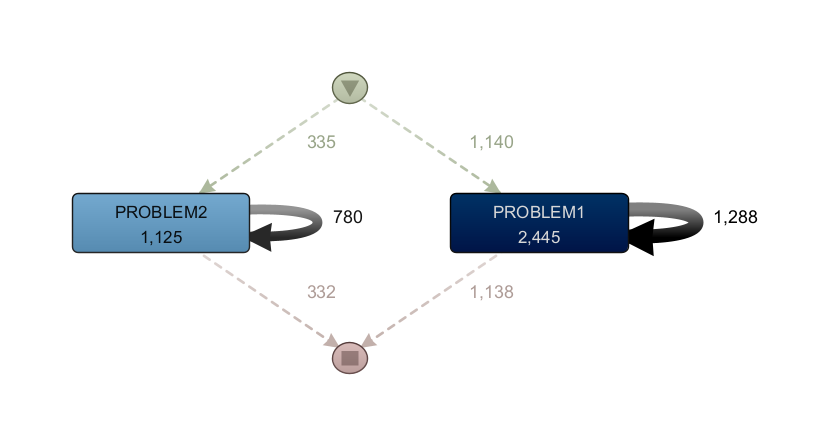
\includegraphics[width=1.10\textwidth, height=0.80\textwidth]{imagenes/DISCO_map/Dataset FusionadoYear1516MidHighGrades.png}
    \caption{Extracción de procesos del dataset integrado por las acciones mapa de los grupos con calificación \emph{``media-alta''} del curso académico 1516.}
    \label{fig:mapYear1516MidHighGrades}
  \end{subfigure}
  \hfill
  \begin{subfigure}[t]{0.60\textwidth}
    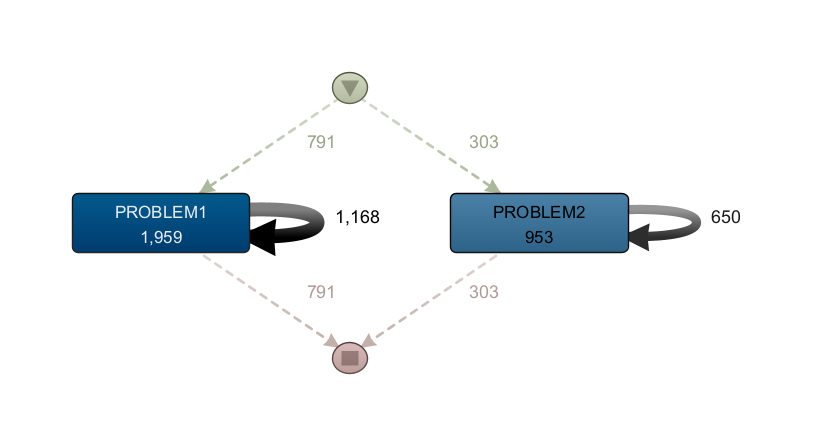
\includegraphics[width=1.10\textwidth, height=0.80\textwidth]{imagenes/DISCO_map/Dataset FusionadoYear1617MidHighGrades.png}
    \caption{Extracción de procesos del dataset integrado por las acciones mapa de los grupos con calificación \emph{``media-alta''} del curso académico 1617.}
    \label{fig:mapYear1617MidHighGrades}
  \end{subfigure}
  \hfill
  \begin{subfigure}[t]{0.60\textwidth}
    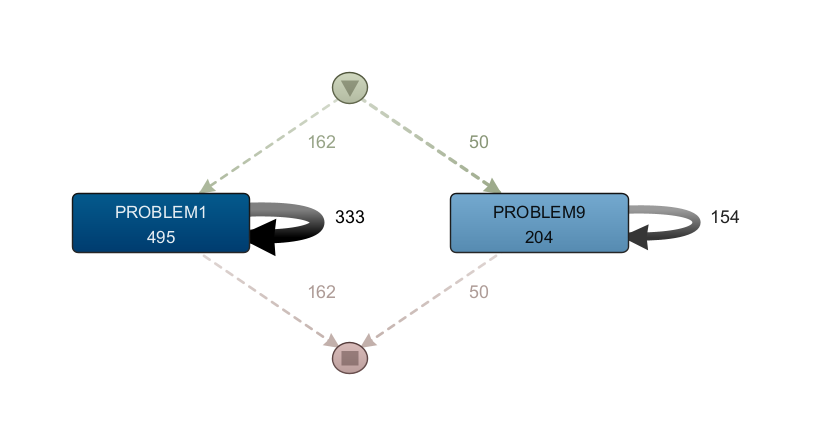
\includegraphics[width=1.10\textwidth, height=0.80\textwidth]{imagenes/DISCO_map/Dataset FusionadoYear1718MidHighGrades.png}
    \caption{Extracción de procesos del dataset integrado por las acciones mapa de los grupos con calificación \emph{``media-alta''} del curso académico 1718.}
    \label{fig:mapYear1718MidHighGrades}
  \end{subfigure}
  \hfill
  \begin{subfigure}[t]{0.60\textwidth}
    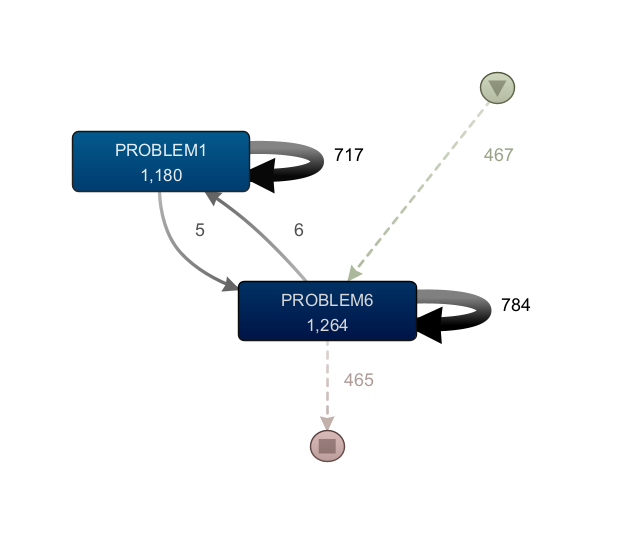
\includegraphics[width=1.10\textwidth, height=1.10\textwidth]{imagenes/DISCO_map/Dataset FusionadoYear1920MidHighGrades.png}
    \caption{Extracción de procesos del dataset integrado por las acciones mapa de los grupos con calificación \emph{``media-alta''} del curso académico 1920.}
    \label{fig:mapYear1920MidHighGrades}
  \end{subfigure}
  \caption{Extracción de procesos del dataset integrado por las acciones mapa de los grupos con calificación \emph{``media-alta''} a lo largo de cuatro cursos académicos.}
\end{figure}

\begin{figure}[H]
  \begin{subfigure}[t]{0.60\textwidth}
    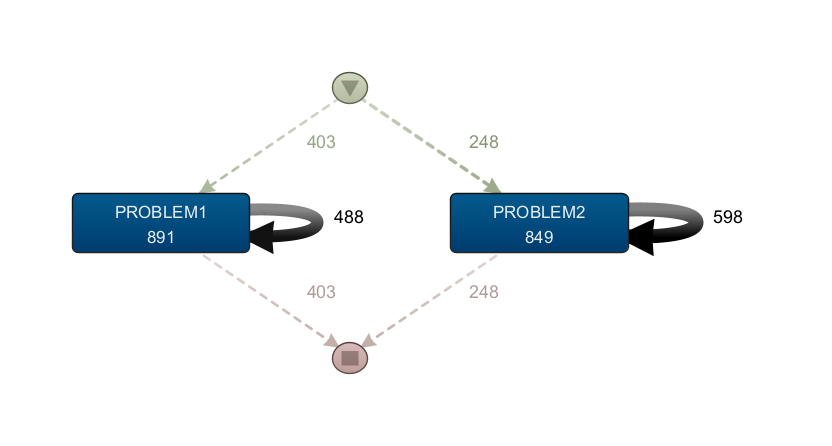
\includegraphics[width=1.10\textwidth, height=0.80\textwidth]{imagenes/DISCO_map/Dataset FusionadoYear1516HighGrades.png}
    \caption{Extracción de procesos del dataset integrado por las acciones mapa de los grupos con calificación \emph{``alta''} del curso académico 1516.}
    \label{fig:mapYear1516HighGrades}
  \end{subfigure}
  \hfill
  \begin{subfigure}[t]{0.60\textwidth}
    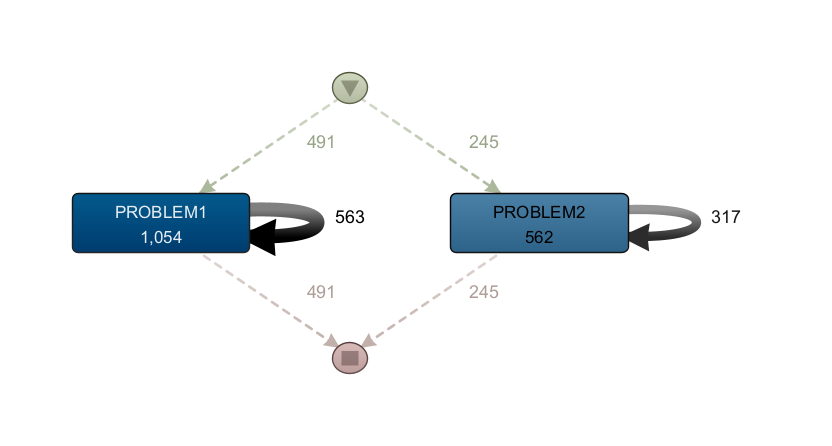
\includegraphics[width=1.10\textwidth, height=0.80\textwidth]{imagenes/DISCO_map/Dataset FusionadoYear1617HighGrades.png}
    \caption{Extracción de procesos del dataset integrado por las acciones mapa de los grupos con calificación \emph{``alta''} del curso académico 1617.}
    \label{fig:mapYear1617HighGrades}
  \end{subfigure}
  \hfill
  \begin{subfigure}[t]{0.60\textwidth}
    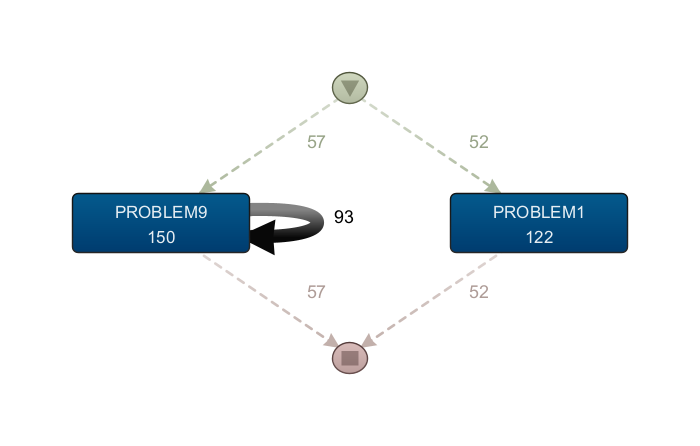
\includegraphics[width=1.10\textwidth, height=0.80\textwidth]{imagenes/DISCO_map/Dataset FusionadoYear1920HighGrades.png}
    \caption{Extracción de procesos del dataset integrado por las acciones mapa de los grupos con calificación \emph{``alta''} del curso académico 1920.}
    \label{fig:mapYear1920HighGrades}
  \end{subfigure}
  \caption{Extracción de procesos del dataset integrado por las acciones mapa de los grupos con calificación \emph{``alta''} a lo largo de cuatro cursos académicos.}
\end{figure}

\begin{figure}[H]
    \centering
    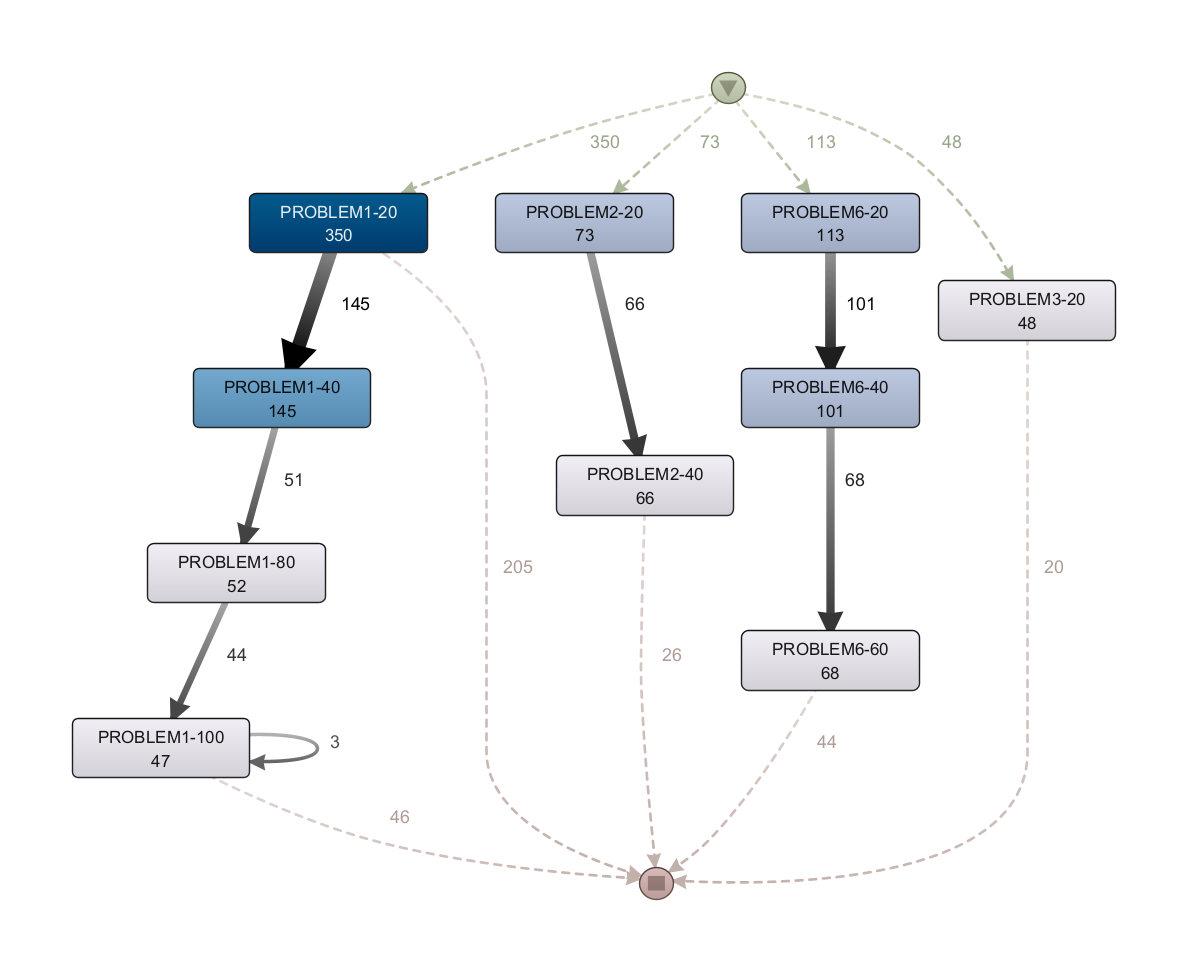
\includegraphics[width=1.25\textwidth]{imagenes/DISCO_compound/Year1617WorstGrades.png}
    \caption{Extracción de procesos del dataset integrado por las acciones compuestas de los grupos con calificación \emph{``baja''} del curso académico 1617.}
    \label{fig:year1617WorstGrades}
\end{figure}

\begin{figure}[H]
    \centering
    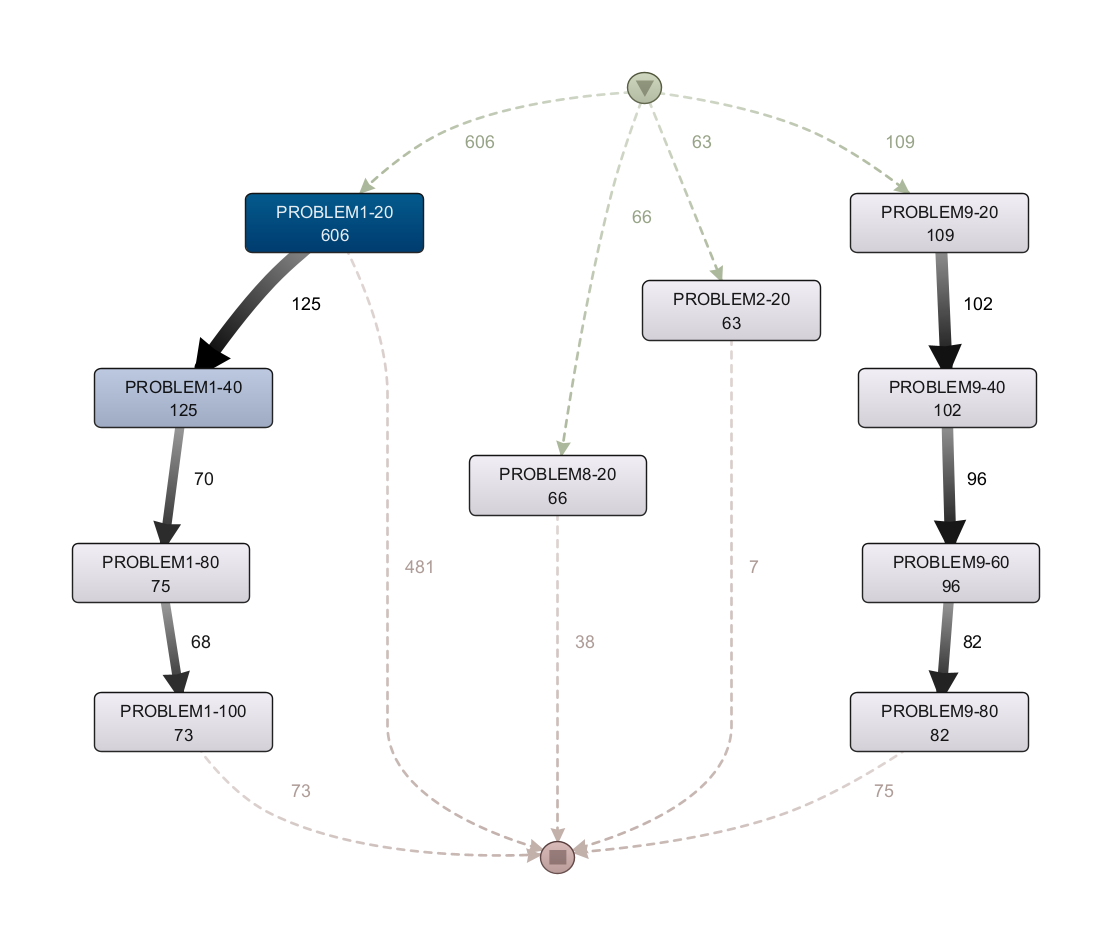
\includegraphics[width=1.25\textwidth]{imagenes/DISCO_compound/Year1718WorstGrades.png}
    \caption{Extracción de procesos del dataset integrado por las acciones compuestas de los grupos con calificación \emph{``baja''} del curso académico 1718.}
    \label{fig:year1718WorstGrades}
\end{figure}

\begin{figure}[H]
    \centering
    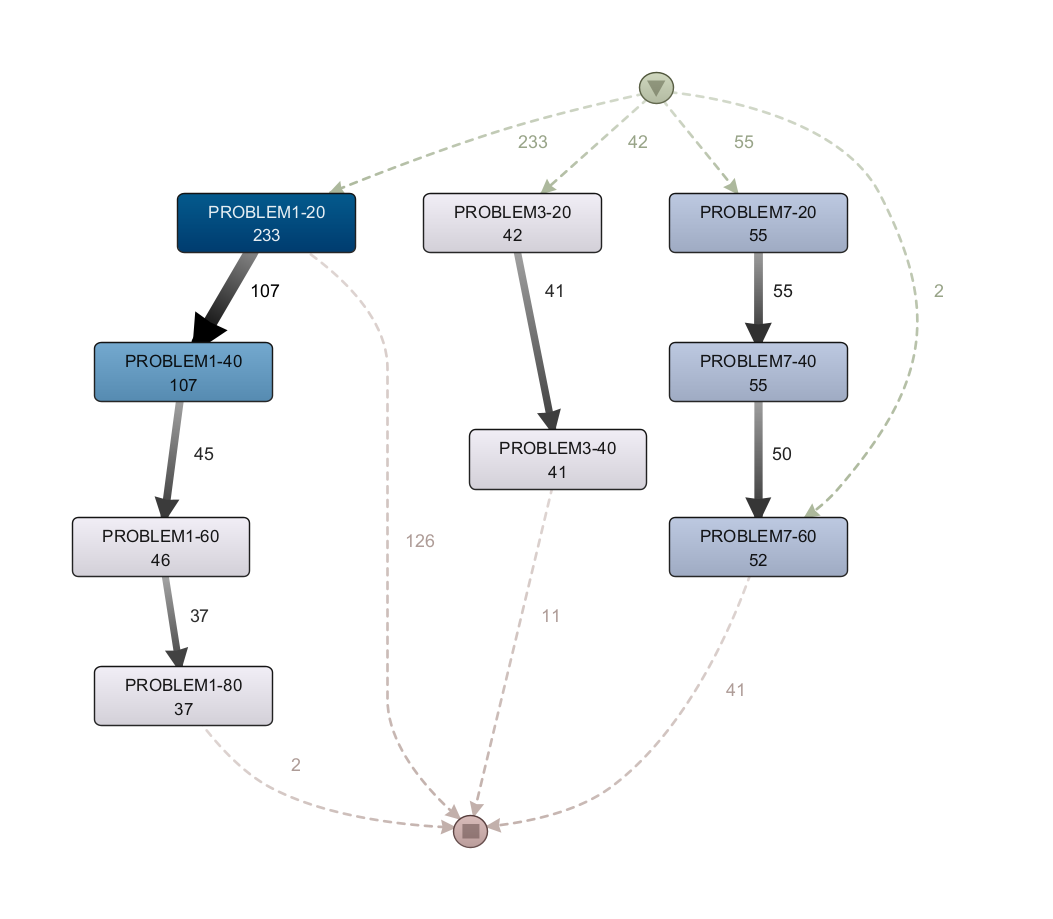
\includegraphics[width=1.25\textwidth]{imagenes/DISCO_compound/Year1920WorstGrades.png}
    \caption{Extracción de procesos del dataset integrado por las acciones compuestas de los grupos con calificación \emph{``baja''} del curso académico 1920.}
    \label{fig:year1920WorstGrades}
\end{figure}

\begin{figure}[H]
    \centering
    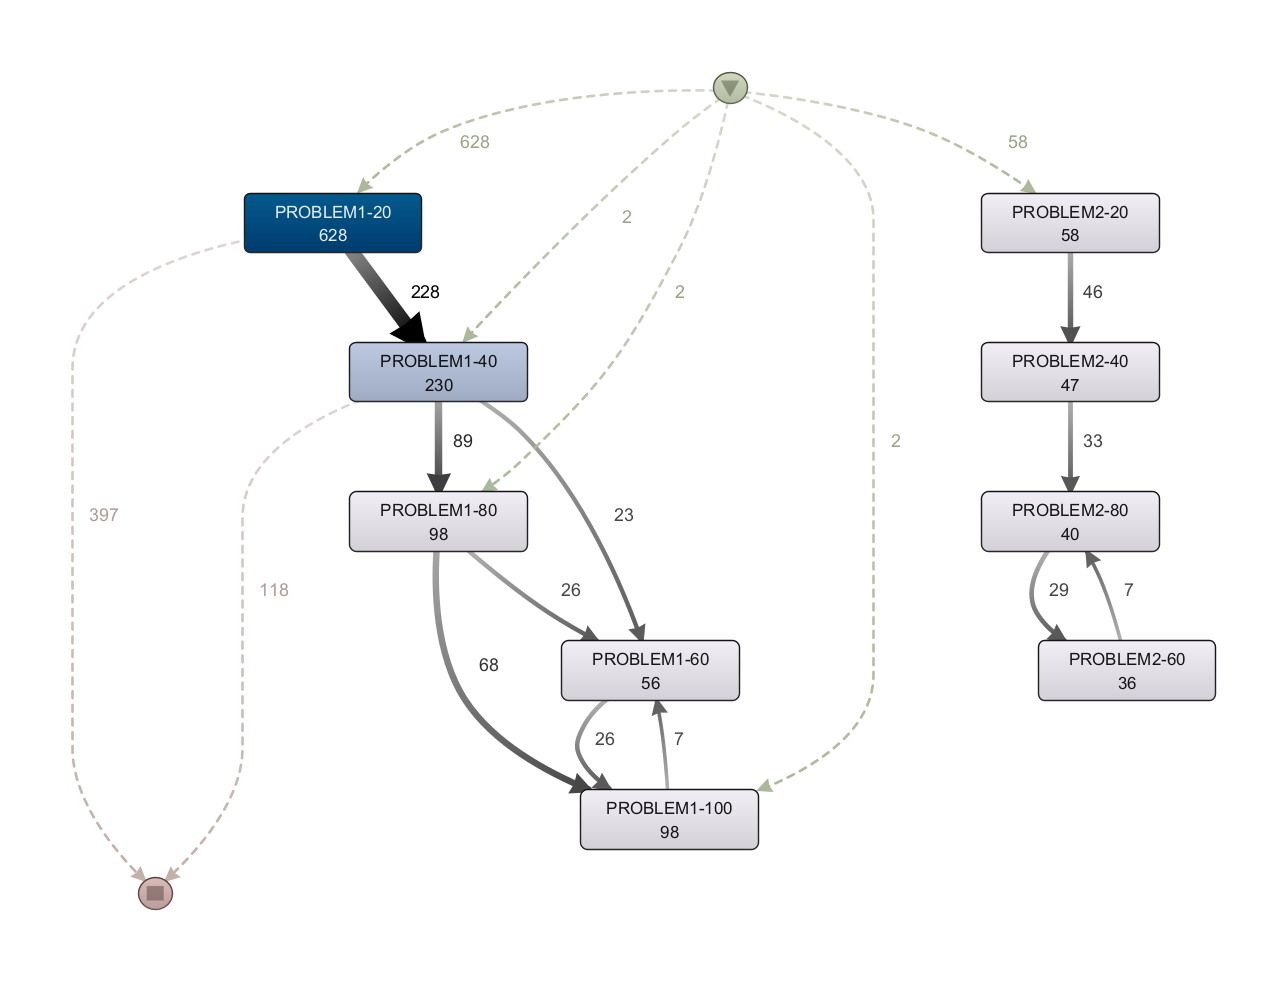
\includegraphics[width=1.25\textwidth]{imagenes/DISCO_compound/Year1516MidLowGrades.png}
    \caption{Extracción de procesos del dataset integrado por las acciones compuestas de los grupos con calificación \emph{``media-baja''} del curso académico 1516.}
    \label{fig:year1516MidLowGrades}
\end{figure}

\begin{figure}[H]
    \centering
    \includegraphics[width=1.25\textwidth]{imagenes/DISCO_compound/Year1718MidLowGrades.png}
    \caption{Extracción de procesos del dataset integrado por las acciones compuestas de los grupos con calificación \emph{``media-baja''} del curso académico 1718.}
    \label{fig:year1718MidLowGrades}
\end{figure}

\begin{figure}[H]
    \centering
    \includegraphics[width=1.25\textwidth]{imagenes/DISCO_compound/Year1920MidLowGrades.png}
    \caption{Extracción de procesos del dataset integrado por las acciones compuestas de los grupos con calificación \emph{``media-baja''} del curso académico 1920.}
    \label{fig:year1920MidLowGrades}
\end{figure}

\begin{figure}[H]
    \centering
    \includegraphics[width=1.25\textwidth]{imagenes/DISCO_compound/Year1516MidHighGrades.png}
    \caption{Extracción de procesos del dataset integrado por las acciones compuestas de los grupos con calificación \emph{``media-alta''} del curso académico 1516.}
    \label{fig:year1516MidHighGrades}
\end{figure}

\begin{figure}[H]
    \centering
    \includegraphics[width=1.25\textwidth]{imagenes/DISCO_compound/Year1617MidHighGrades.png}
    \caption{Extracción de procesos del dataset integrado por las acciones compuestas de los grupos con calificación \emph{``media-alta''} del curso académico 1617.}
    \label{fig:year1617MidHighGrades}
\end{figure}

\begin{figure}[H]
    \centering
    \includegraphics[width=1.25\textwidth]{imagenes/DISCO_compound/Year1718MidHighGrades.png}
    \caption{Extracción de procesos del dataset integrado por las acciones compuestas de los grupos con calificación \emph{``media-alta''} del curso académico 1718.}
    \label{fig:year1718MidHighGrades}
\end{figure}

\begin{figure}[H]
    \centering
    \includegraphics[width=1.25\textwidth]{imagenes/DISCO_compound/Year1920MidHighGrades.png}
    \caption{Extracción de procesos del dataset integrado por las acciones compuestas de los grupos con calificación \emph{``media-alta''} del curso académico 1920.}
    \label{fig:year1920MidHighGrades}
\end{figure}

\begin{figure}[H]
    \centering
    \includegraphics[width=1.25\textwidth]{imagenes/DISCO_compound/Year1516HighGrades.png}
    \caption{Extracción de procesos del dataset integrado por las acciones compuestas de los grupos con calificación \emph{``alta''} del curso académico 1516.}
    \label{fig:year1516BestGrades}
\end{figure}

\begin{figure}[H]
    \centering
    \includegraphics[width=1.25\textwidth]{imagenes/DISCO_compound/Year1617HighGrades.png}
    \caption{Extracción de procesos del dataset integrado por las acciones compuestas de los grupos con calificación \emph{``alta''} del curso académico 1617.}
    \label{fig:year1617BestGrades}
\end{figure}

\begin{figure}[H]
    \centering
    \includegraphics[width=1.25\textwidth]{imagenes/DISCO_compound/Year1920HighGrades.png}
    \caption{Extracción de procesos del dataset integrado por las acciones compuestas de los grupos con calificación \emph{``alta''} del curso académico 1920.}
    \label{fig:year1920BestGrades}
\end{figure}

\section{Análisis de los procesos con segmentación}
\subsection{Arquitectura del software}

\subsection{Ejecución del software}
Para la correcta ejecución del software se han de seguir las siguientes indicaciones:
\begin{itemize}
\item En primer lugar, se ha de ejecutar el makefile para compilar el código C++ que se encuentra en la carpeta \texttt{/code/C++/DAG}.
\item A continuación, para obtener los resultados a partir de los diferentes archivos .csv que obtuvimos en esta iteración y en iteración anterior se deberá ejecutar el script que se encuentra en ese mismo directorio.
\end{itemize}

\section{Análisis de los motivos en los cambios de comportamiento}
\input{capitulos/capitulo_06/iteracion_3}

\section{Análisis de si hay cambios inducidos por los éxitos de los demás grupos}

%
%\input{capitulos/07_Pruebas}
%
%\input{capitulos/08_Conclusiones}
%
%%\chapter{Conclusiones y Trabajos Futuros}
%
%
%%\nocite{*}
%\bibliography{bibliografia/bibliografia}\addcontentsline{toc}{chapter}{Bibliografía}
%\bibliographystyle{miunsrturl}
%
%\appendix
%\input{apendices/manual_usuario/manual_usuario}
%%\input{apendices/paper/paper}
%\input{glosario/entradas_glosario}
% \addcontentsline{toc}{chapter}{Glosario}
% \printglossary

\chapter*{}
\thispagestyle{empty}

\end{document}
